\chapter{Results: From Specification to End Product}
\label{ch:game}
\containsfigures{Results: From Specification to End Product}
\containslistings{Results: From Specification to End Product}
\containstables{Results: From Specification to End Product}

\chapterepigraph{Finishing races is important, but racing is more important.}{Dale Earnhardt}

% introduction for this chapter, is not a section



% introduction
% ------------
Our project, irrelevent to implementation language has a very simliar foundation to all games, requiring networking between computers playing the game, graphics engine that can draw the game, assets/sprites for in game entities.

The game's implementation will be designed with an infrastructure that is at the core. All game features will run on top of this infrastructure, having little dependency on other game features, but having complete dependency on the infastrcture. This architecture allows very module design with regards to game features, allowing new game features to be added to the implementation only a slight modification of the infrastructure to include the new feature. By designing the architecture like this, It faciliates a release based schedule.

A high level specification is now available that specifices the elemnts of the game. To bring this high level specification to reality, the game design will be broken down into 3 major releases: Alpha, Beta 1, and Beta 2. Each release specifies the game features that must be in the game. Essentially the game design is broken down into game features, with higher priority game features being specified in earlier releases.
Alpha Release is primarily focused on building the game's Infrastructure, this is the core of the game with all the back end logic that is never seen by the player. By the end of Alpha 1 the game infrastructure is mostly complete, and the game is in a state where game logic can now be added on like modules with little dependency 
Beta 1 and Beta 2 are both game feature oriented, building on top of the existing infrastructure, adding features described in the specification. These releases will heavily focus on meeting the specification's specified game features.

% Laying The Foundation
% ---------------------
Terminology was the first step in the conversion process from specification to working game. 
An initial ambiguity was that many of haskell libraries being looked into had a concept of 'world' which varied dramatically, which in term caused every member of the team to have a different meaning for the word. This caused many misunderstandings until an internal terminaology was devised within the team to describe common terms such as 'client state'. Once the terminology hurdle was solved, The team was able to share design ideas efficiently.

By the end of alpha Stage a working 'game' was needed, somethat that could be used as a base to start adding game features.

The infrastructure must provide a platform that the game features can be implemented ontop of, Hence it must contain:
\begin{itemize}
\item Server-Client communication
\item Rendering capabilities for assets
\item Game loop
\item Model of game components
\end{itemize}

Mistakes at this stage will cost heavily later down the line, because so much will dependend on the infrastructure. 

\begin{comment}

alpha stage layout
------------------
features wanted at this stage:
    - networking
    - server client loop
    - game update model (lock-step no no no)
    - ship move orders
    - world rendering(easy debugging)
    - more focus around infrastructure than features
    
    
  - lack of libraries, implemeintg our own networking, GUI library.
  - implementation of network library.
  - server and client not distinquished just yet
  - game loop
  - lock-step big part
    - arguments for and against
  - integration of assets into game
  - API for game how entities are added
  - how generating diffs will work

  - infrastructure components
    - networking
    - gameploop
    - how the server and client synchronize
    - graphics


\end{comment}


% sections
\clearpage
\section{Server-Client Synchronisation}

\newcommand{\stepOneName}{lockstep}
\newcommand{\stepTwoName}{simple server client}
\newcommand{\stepThreeName}{server client with simulation}

% topology of network(star diagram, what server does, what client does)
\begin{marginfigure}
	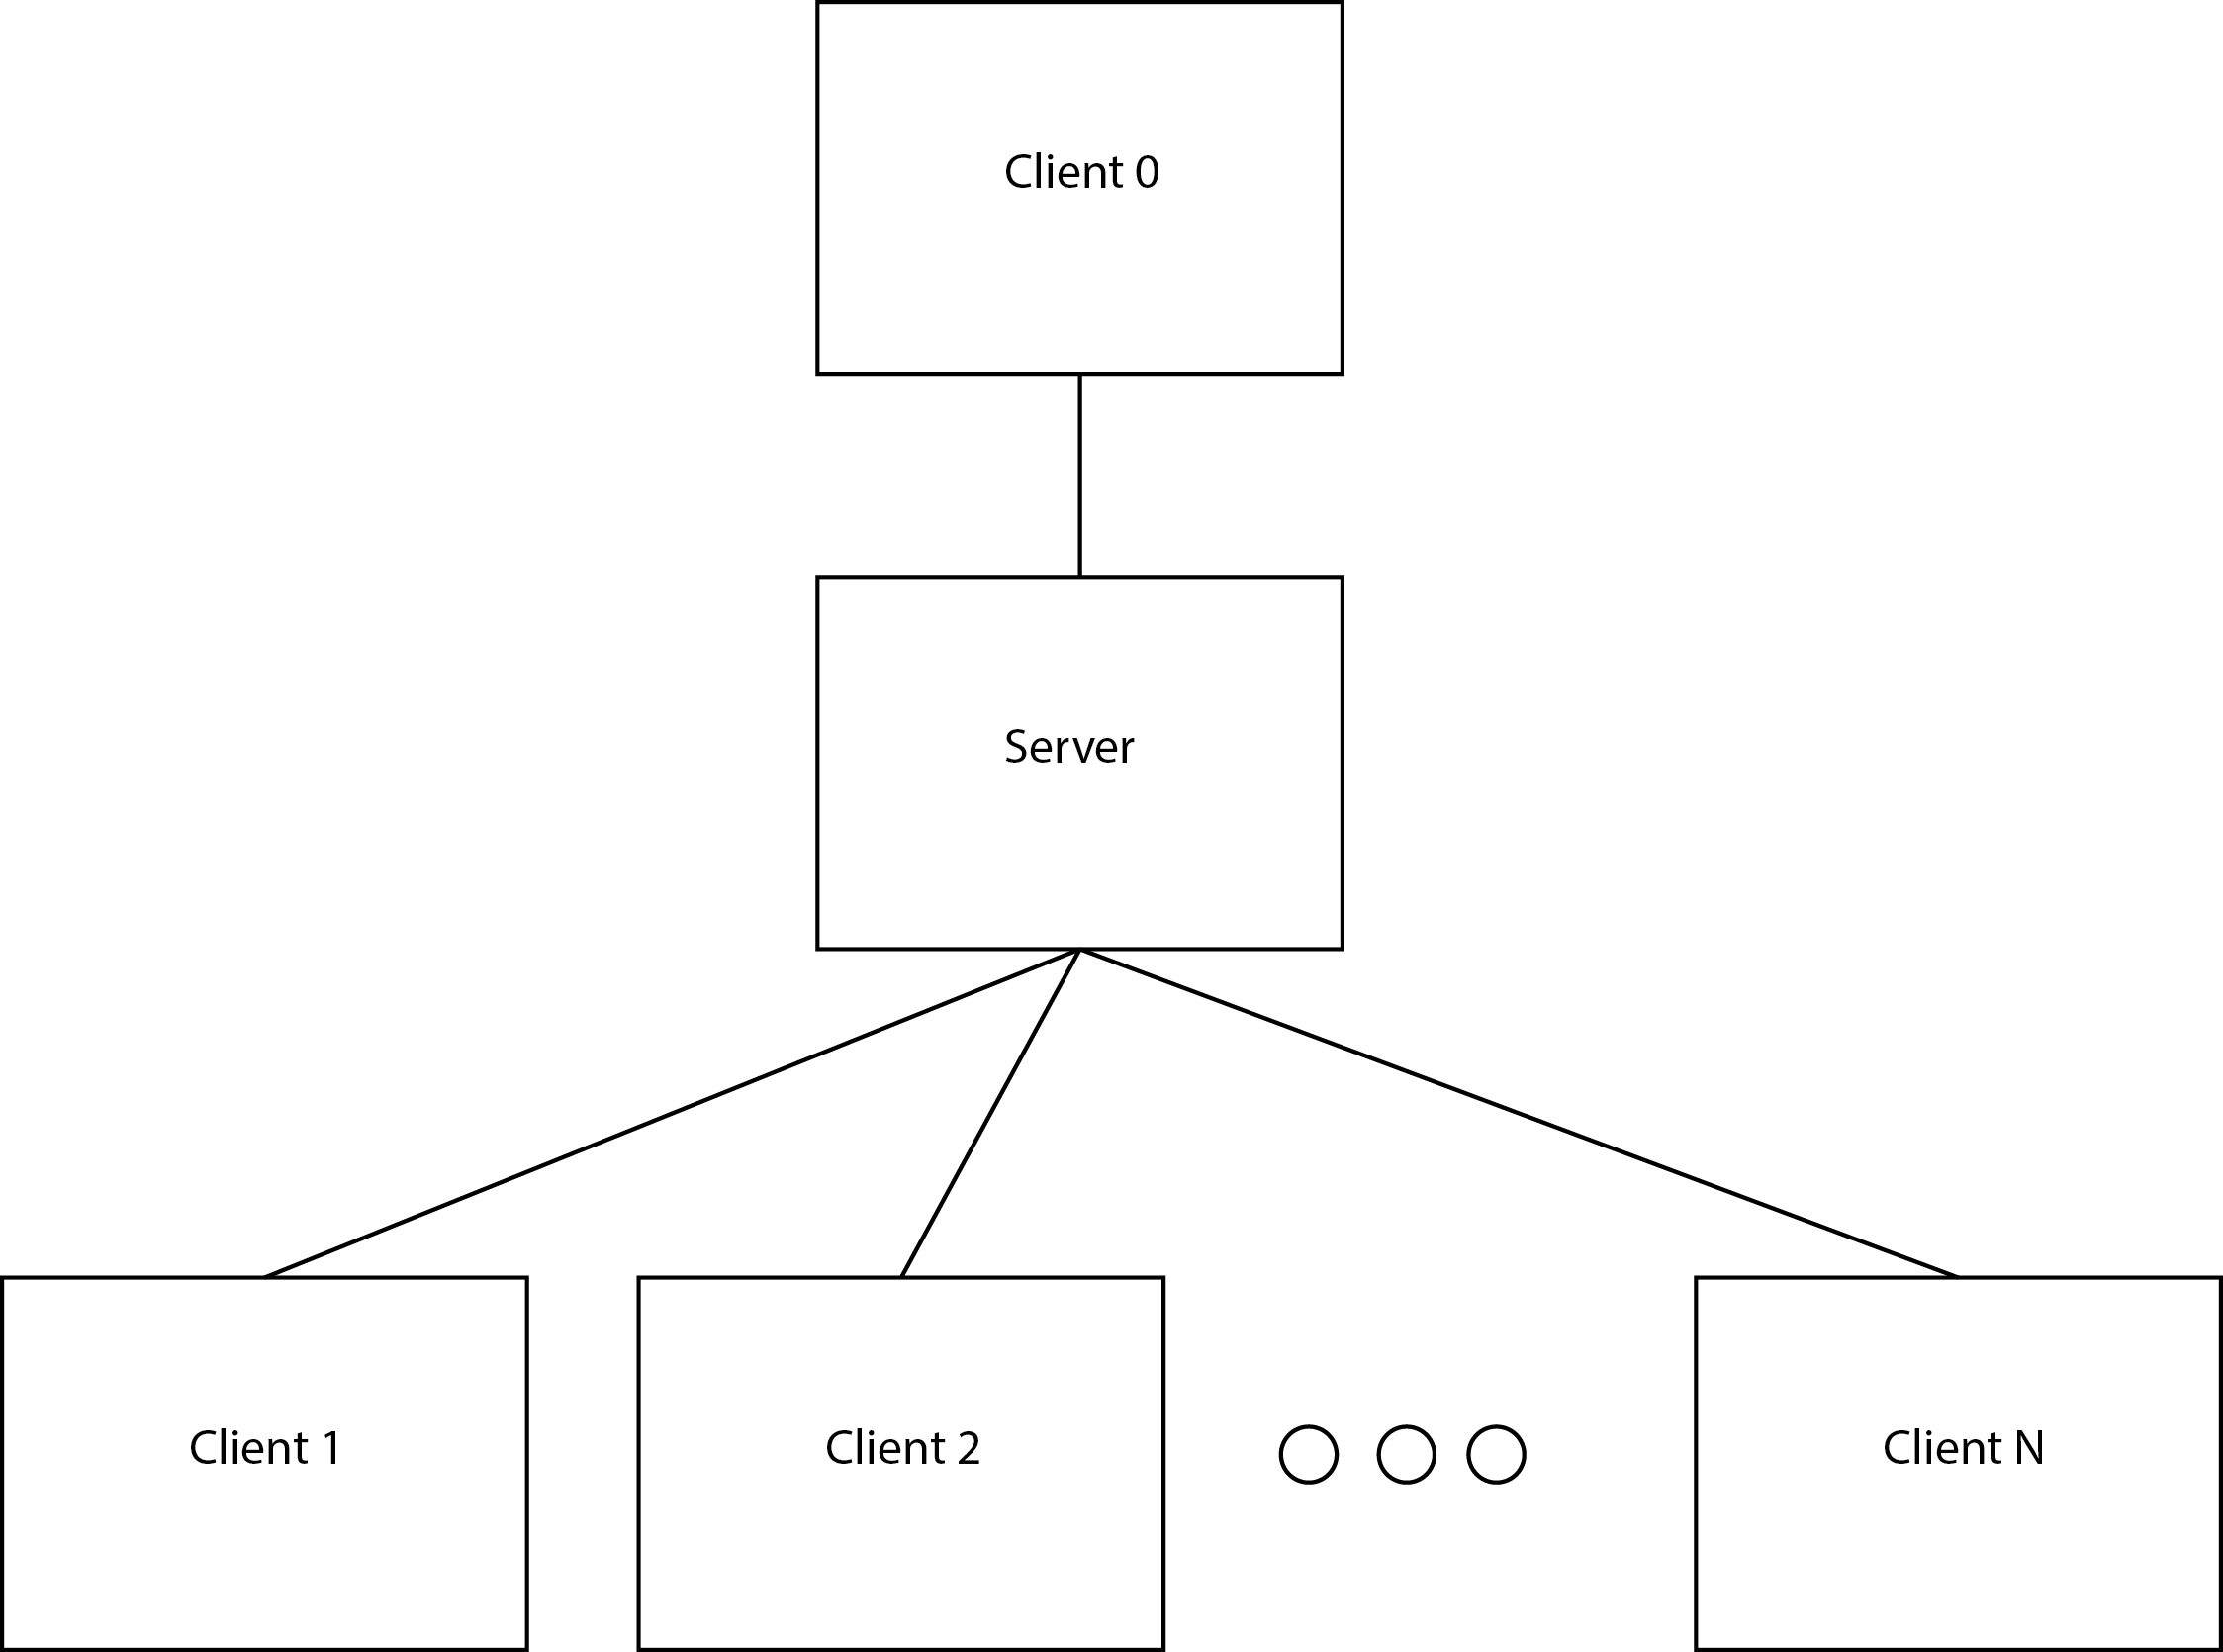
\includegraphics{res/computer_communication_architecture/NetworkTopology.png}
	\caption{
	network topology for multiplayer.
	}
	\label{fig:serverClientSychNetworkTopology}
\end{marginfigure}

The topology is a typical Star Network, with server in centre, and all clients only connecting to server.
There are $N+1$ player connected, where client 0 is the client that is hosting the server.
Since client 0 is hosting the server, they have special permissions to stop the server at any point, ending the game.
This topology greatly simplifies the requirements of the networking, because every client has to only connect to server, and receive all its updates from 1 single place. 

% protocol for synching game states between client server (command, update)
Figure \ref{fig:loops} gives a good representation how the server and a given client communicate.
Both the server and client have a full copy of the model representing the game state.
Their were a variety of benefits from this, the least of which it allowed the clients to scroll around the map without requiring any network traffic.

When the player gives an order, i.e. to move a ship to a given destination, that order is sent to the server in the form of a command.
On the server side, that command is used to 'update' the server's game model. Now the server's game state is at a later version than the clients. The server generates updates that can be applied to all client's game states to bring them to the same version as the server's version.

An example of an update message is: A ship has been given a move order to a location on opposite side of map.
Since their is no simulation on the client side, the ship will only move if the server sends an position update to the clients, moving it slightly closer to its destination. This means that for every time step, every ship that is moving will require an update message send across the network to every client. 

The move update will look something like this:

\begin{margintable}
    \begin{tabular}{l l l l l}
    \toprule
    \emph{shipID} & \emph{x} & \emph{y} & \emph{direction x} & \emph{direction y} \\ 
    \midrule
    43 & 10 & 15 & 0 & 1 \\
    \bottomrule
    \end{tabular}
    	\vspace{1em}
	\caption{example of a position update message}
	\label{tab:positionUpdateExample}
\end{margintable}

Instead of the server telling the client where the ship's destination is, and letting the client move the ship their, the server tells the client when to the next jump location. In the example in Figure \ref{tab:positionUpdateExample} the ship with ID 43 has been given a position update to the new coordinates (10,15), facing North which is (0, 1).

Their are a variety of updates message, depending on which part of the game needs to be updated. 
Originally there was only 3 types of updates:
\begin{description}
\item[addEntity] used for adding an entity to the game. It contains the entity being added to the game.
\item[deleteEntity] used for deleting an entity. An example of use would be when an entity was just blown up. Only contains the entiyID
\item[updateEntity] most common update, used to update an entity. It contains the new entity, and the existing entity is replaced with the entity inside this update.
\end{description}

Having 3 updates provided a very simple design. 
2 out of the 3 updates(addEntity and updateEntity) contains an entity object which is very large in size.
To send an entity object across the network can be very slow and should only be done when necessary.

The addEntity update needs to contain an entity because that entity is currently not in the game, so all the fields of the entity need to be sent across to all the clients. Since addEntity is primarily used at the start of a game when all the entities are loaded into the game, this is not a problem.

However the updateEntity update is sent every time an entity changes location, direction, targets, etc.
Each time an entity's field changes the entire entity must be sent across the network to all the clients.
Not only is this taking up a large amount of bandwidth, but it is sending a large proportion of redundant fields which haven't been changed.
The solution to this was to split the updateEntity update into multiple updates, each one for a common update usage.
The different types of updates to an entity were identifies and a new update message was given to it. 
Table \ref{tab:updateMessageTypes} contains the update messages devised.

\begin{table}
    \begin{tabular}{p{5em} p{15em} p{6em}}
    \toprule
    \emph{Update Type} & \emph{Description} & \emph{Fields} \\
    \midrule
    position & used when both the ship's location and direction has changed & entityID, location, direction \\
    order & when a ship's orders change & entityID, order \\
    goal & when a ship's goal changes & entityID, goal \\
    plan & when a ship's plan to achieve its goal changes & entityID, plan \\
    health & when a ship's hull or shields health changes & entityID, hull health, shield health \\ 
    \bottomrule
    \end{tabular}
    	\vspace{1em}
	\caption{each type of update message, description of its usage, and the fields it will contain}
	\label{tab:updateMessageTypes}
\end{table}

Now, when a ship's field, say direction changes, the direction update message is used instead of the old entity update message.
This is significantly cheaper with regards to network usage because only the ship's ID and new location are sent.

% network traffic calculation
Their were concerns that the volume of traffic required to maintain all the client's game states updates would still be too great for a playable game.
Therefore a traffic analysis was done to estimate how much network traffic would actually be required.
When assumptions are made concerning the game, such as number of ships, number of game steps per second, etc, worst case scenario will be assumed giving the limitations of the game, IE we will know the maximum number of ships the game can have before the game becomes effects by network bandwidth.



The size of each update message will need to be estimated as well as how frequently that message will be sent.

First, the size of field types will need estimating using language independent types such as int, float, double, etc.
This is done in Table \ref{{tab:positionUpdateExample}
\begin{margintable}
    \begin{tabular}{p{5em} p{5em}}
    \toprule
    \emph{Field Type} & \emph{Field Size/bytes} \\
    \midrule
    int & 4 \\ 
    long & 8 \\ 
    float & 4 \\
    double & 8 \\    
    \bottomrule
    \end{tabular}
    	\vspace{1em}
	\caption{example of a position update message}
	\label{tab:positionUpdateExample}
\end{margintable}

Now we have estimates of size for the different types, we can assign types to the fields of the message

\begin{margintable}
    \begin{tabular}{p{5em} p{5em} p{5em}}
    \toprule
    \emph{Field Name} & \emph{Size/bytes} \\
    \midrule
    entityID & 4 \\ 
    location & 8 \\
    direction & 8 \\ 
    order & 15 \\
    goal & 9 \\ 
    plan & 100 \\ 
    hull & 4  \\ 
    shield & 4  \\  
    \bottomrule
    \end{tabular}
    	\vspace{1em}
	\caption{example of a position update message}
	\label{tab:positionUpdateExample}
\end{margintable}



For the plan field, it was assumed that each action within the plan was approximately 20 bytes, and that the average plan has 5 steps.

The following table estimates the size of a message to sent across network:
\begin{center}
    \begin{tabular}{| l | l | l |}
    \hline
    Update Type & size / bytes & frequency per game step \\ \hline
    position & 20 & 1 \\ \hline
    order & 19 & 0.2 \\ \hline
    goal & 14 & 0.3 \\ \hline
    plan & 104 & 0.3 \\ \hline
    health & 12 & 0.1 \\ 
    \hline
    \end{tabular}
\end{center}


Now we have the size and frequency of each update message, we can calculate how many bytes are sent to a single client every game step. 
$$ bytes = 20*1 + 19*0.2 + 14*0.3 + 104*0.3 + 12*0.1 $$
$$ bytes = 60.4 $$

We have $S$ representing the number of game steps per second, and $N$ representing the number of clients connected to server.
The number of bytes the server sends per second is
$$ bytes = S * N * 60.4 $$

We now have a formula to calculate network traffic, we need to apply to to various values of $N$ and $S$.

% s=15, 30, 45, 60, n =2, 4, 8, 16
\begin{center}
    \begin{tabular}{| l | l | l |}
    \hline
    S & N & kB/second \\ \hline
    15 & 2 & 1.77 \\ \hline
    \hline
    \end{tabular}
\end{center}

-------------------------- worked upto here ------------------


constants for calculation:
\begin{center}
    \begin{tabular}{| l | l |}
    \hline
    Constant & Value \\ \hline
    world updates / second & 30 \\ \hline
    ships & 40 \\
    \hline
    \end{tabular}
\end{center}

A 

The next step was to calculate the size of a ship update message.

Hence a single ship movement update message would be:
$$ size = (shipID, x, y, directionX, directionY, hullHealth) = 5 * 4 bytes = 20 bytes $$
To send a single ship update to a single client is 20 bytes.



			world updates per second 30
			ships in world = 40
			bullets in world = 1000
			ship movement update = (shipId, x, y, direction) = 4 * 4bytes = 16 bytes.
			bullet movement update = (bulletId, x, y, direction) = 4 * 4bytes = 16bytes
			per client:
				per update:
 					ship data = 40 * 16bytes = 640bytes
					bullet data = 1000 * 16bytes = 16000bytes
					total data = 16640bytes
			    per second = 30 * 16640 = 499200bytes = 487.5KB/S
			3 clients = 3 * 487.5KB/s = 1462.5KB/s = 1.43MB/s

% advantages/disadvantages of lockstep
% advantages/disadvantages of server client with simulation


\begin{comment}

This section talks about how multiplayer was achieved.
This includes the network topology.
server-client allows master copy to exist on server.

- master copy of world on server
- clients perform no logic, only apply updates to
- 




----------------------------------- old gay -----------------------------------------

we need to work out how the computers talked to each other very early on
2 considerations: peer 2 peer, client-server
  - advantages of peer 2 peer
  - advantages of peer server-client
  - why server-client chosen 
  - issues experienced with server-client
    - jumpy ship movements
\end{comment}

The game was designed around being multiplayer, so our first goal was to decide how the player's computers would talk to each other.
Since their was an arbitrary number of players (greater than 1), We needed a system that would scale, but would also be robust.
The game was expecting all players to be on the same LAN (Local Area Network), hence a high bandwidth was available for the communications.

There are 3 strategies for the interactions between computers:
\begin{itemize}
\item \stepOneName
\item \stepTwoName
\item \stepThreeName
\end{itemize}


\begin{marginfigure}
	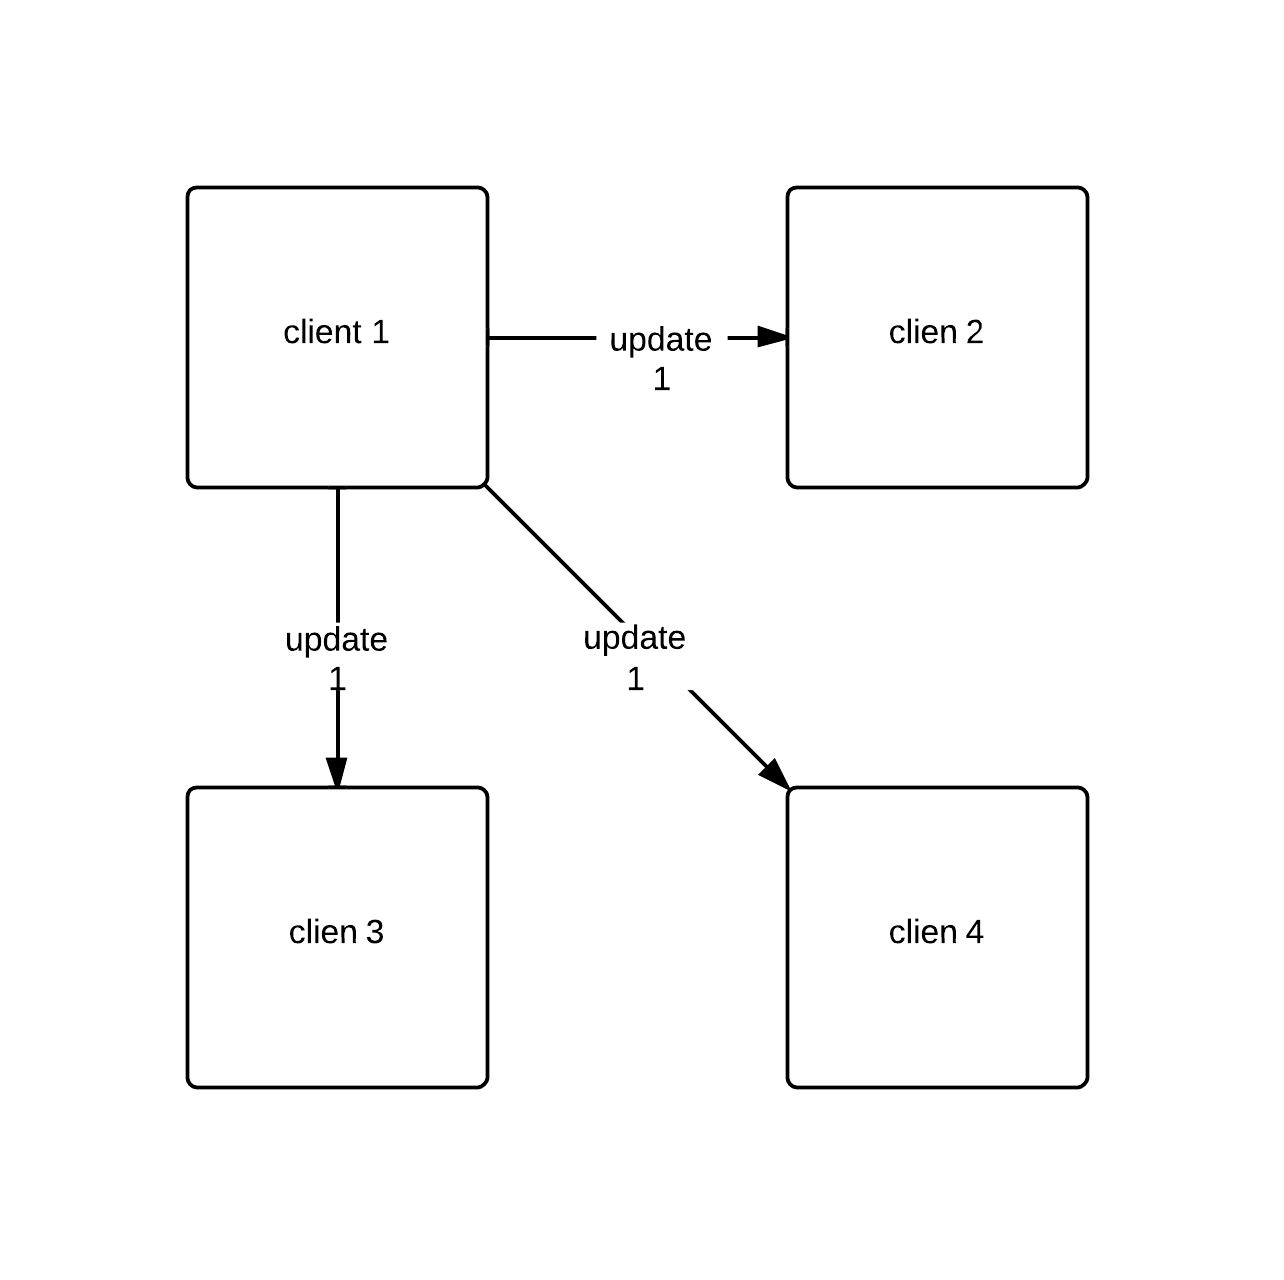
\includegraphics{res/computer_communication_architecture/ServerClientSynchronizationP2P.png}
	\caption{
	\stepOneName : 4 clients connected. client 1 has just modified its game state, so it send the update to all other clients.
	}
	\label{fig:serverClientSychP2P}
\end{marginfigure}

% what
\stepOneName is a peer to peer strategy, in which each computer has a full model of the game. Figure \ref{fig:serverClientSychP2P} shows an example of this strategy. 
Their are 4 computers within game. Each client (client 1, client 2, client 3, and client4) have a full copy of the game.
When client 1 updates performs some actions, they must update their game state, and send this update to all other clients.

\begin{marginfigure}[-30em]
	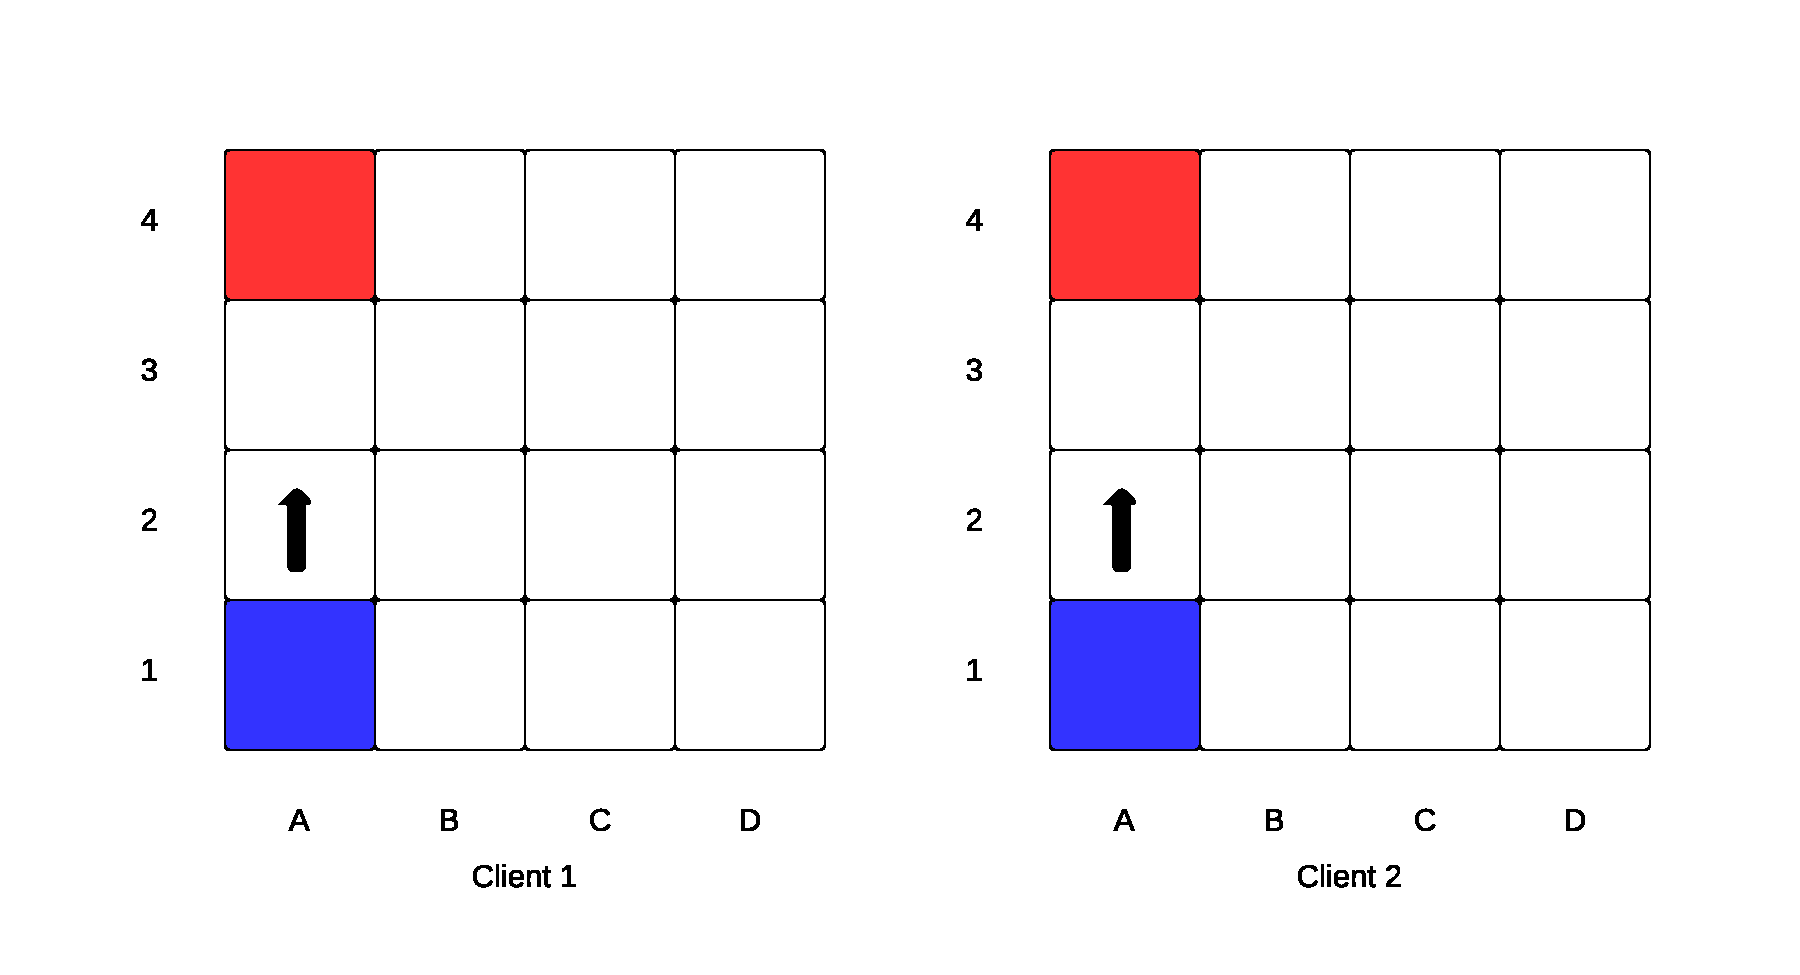
\includegraphics{res/computer_communication_architecture/ServerClientDesynchronisation1.pdf}
	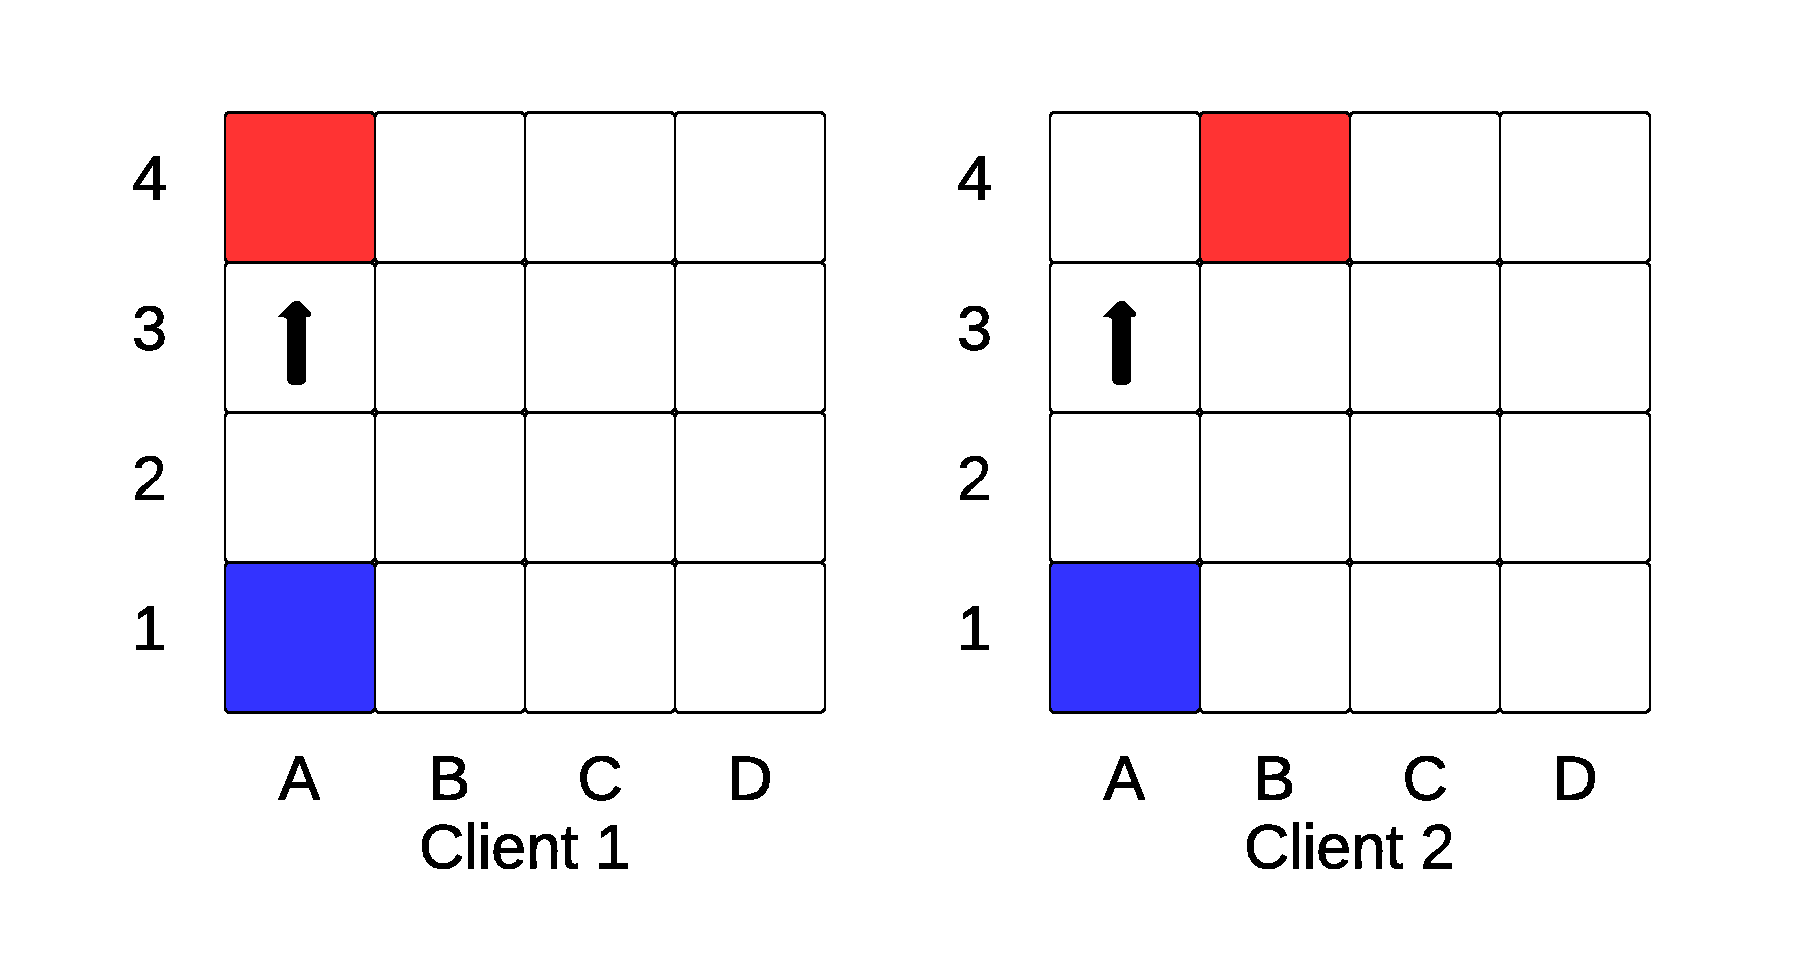
\includegraphics{res/computer_communication_architecture/ServerClientDesynchronisation2.pdf}
	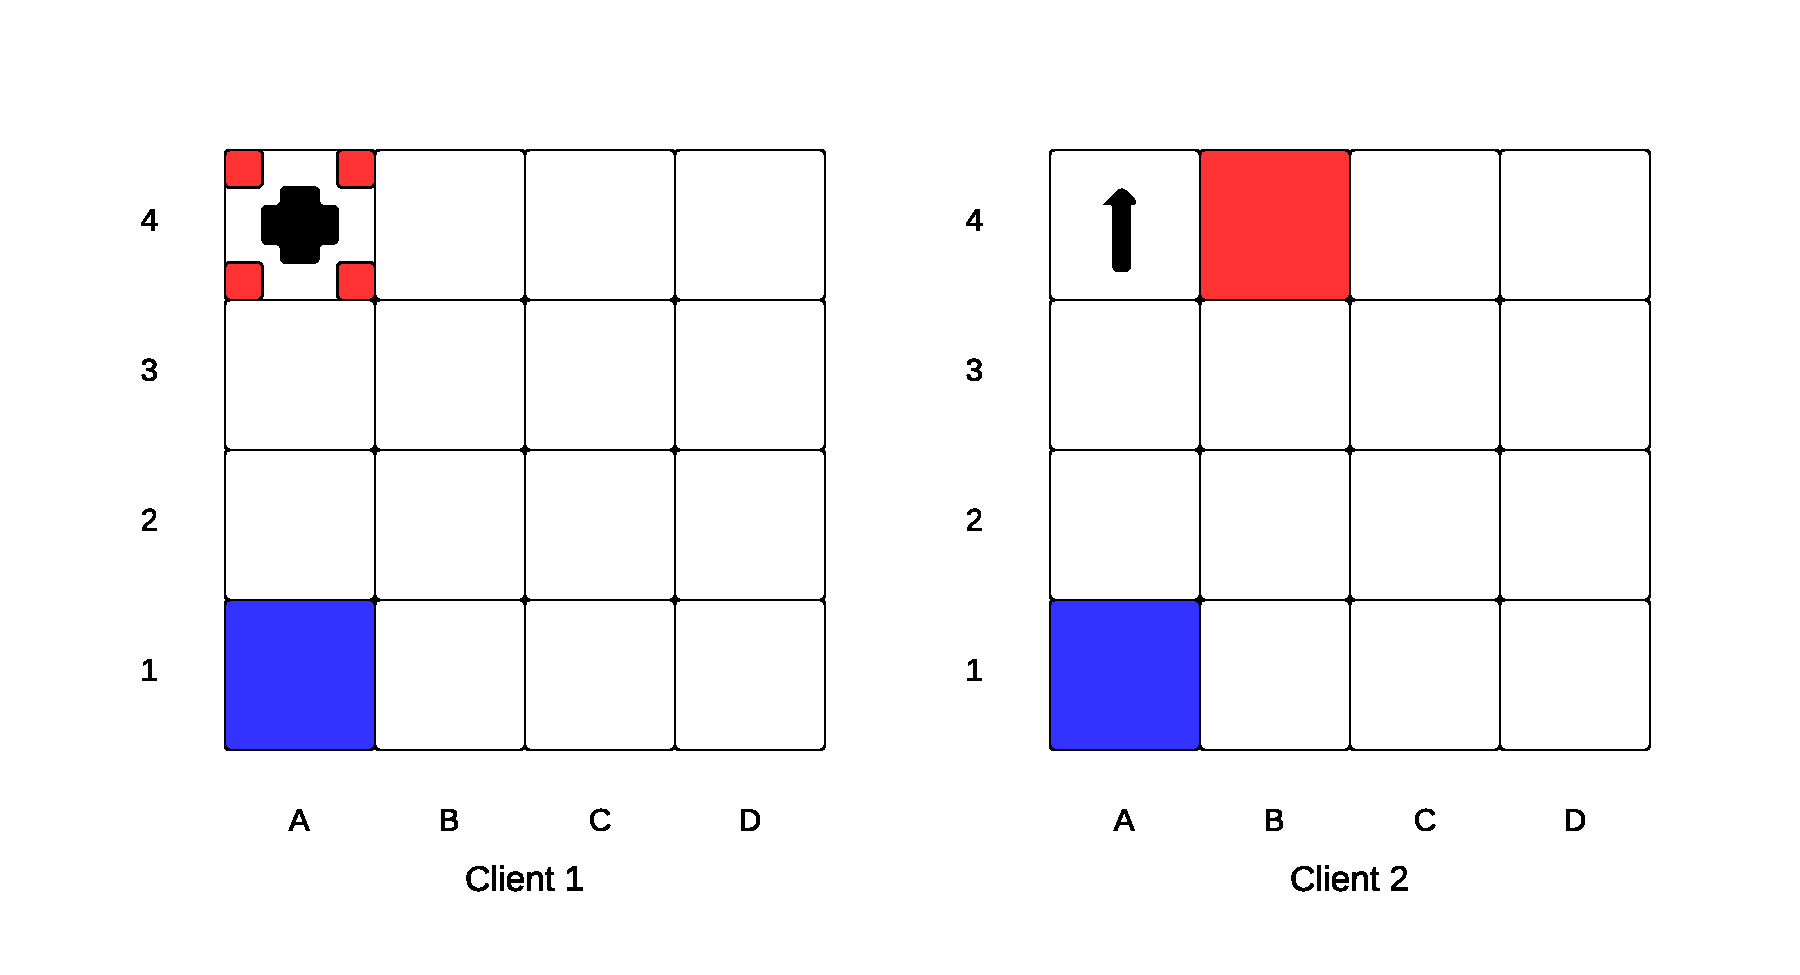
\includegraphics{res/computer_communication_architecture/ServerClientDesynchronisation3.pdf}		
	\caption{
	\stepOneName : example of desynchronization when using the \stepOneName strategy. Client 1 on left, client 2 on right. 
	Each diagram represents state of game for that clients at a given time period.	3 diagrams vertically aligned, First one is top, second one is middle, third one is bottom.
	}
	\label{fig:serverClientDesync}
\end{marginfigure}

% advantages
%   playable with slow networks
This strategy means players can continue to play games on networks with high latency, without any lag. When packets are delayed, the client can continue to play the game, and the game is updated when the packet arrives.
%   no dedicated server required
No client is picked to act as server, which causes game to end if that selected client disconnects.
Since all clients act as server, any client can disconnect and the game continues, providing more robustness which is highly desirable for games with long game intervals, such as Civilization series\cite{civilizationInMyPants}.



% disadvantages
%   disynchronization
Maintaining synchronisation when using a peer-2-peer protocol can be very challenging from a technical point of view, with non-determinism being caused by messages being received by clients at different times causing race conditions.
When this happens in a game, it can cause clients game states to desynchronise.
For example, In Figure \ref{fig:serverClientDesync}, there are 2 clients.
%   corrupted client can effect the entire game



% res/computer_communication_architecture




% lockstep
%   - each client has the master copy of the world
%   - when a client does something, it tells all others
%   - problems:
%     - desycnhronization
%     - currupted client fucks up everyone

% simple server client
%   - it's what we've implemented
%   - no simulation on clients
%   - 1 server that has master copy
%   - server does all processing and sends updates to clients
%   - clients just render the world and send commands to server

% server client with simulation
%   - similar to simple server client but client does 'some' simulation. They in no way can effect the world.
%   - for instance if client knows ships destination and current location it can render the ship graciously moving instead of jumping on every update.


\clearpage\section{Rendering the Game}

% old assets
% ----------
% ships made to look very big
% many prototypes
% merging assets with code, dynamic color

% master copy of assets in dropbox under 4y project/laith/design

One very important aspect of the client program is rendering the current game state to a display for the user to interact with. Creating a picture of the game to display requires a number of graphical assets to visually represent the various entities and scenery that make up the game world. For Project Serenity all of these graphics were created from scratch using Photoshop and Illustrator. Figure~\ref{fig:assets} shows a selection of some of the assets that were created for different entities.

% TODO INSERT FIGURE OF PLANETS AND SHIPS
% full page on planets, full ships

% TODO Chat about the actual rendering process. Thoughts:
%
% * World coordinates: all entities are located in world coordinates and a view of the world is drawn in this way first
% * Viewport: the display is scaled and translated by the current settings stored by the client
% * Along with the actual world there is some extra GUI that helps the player understand the current state of the game:
%      - Minimap
%      - Currently selected entity

The client uses these assets to draw the sector and place each player's ships in the correct locations. This is done by placing the assets using world coordinates in the 2D space defined by the dimensions of the sector.

% TODO Talk about parallax because it's interesting? (Innovative?)

Another interesting piece of the rendering puzzle was to choose a colour as a unique visual representation for each player. This would be used to help players differentiate their ships from the enemy and to identify the planets that they own. A clever algorithm was used that would take a numerical player identifier and return a unique colour:\cite{ankerl2009}

\begin{equation*}
	colour(i) = HSV(i \times \phi^{-1} \mod 1, 1.0, 0.8)
\end{equation*}
\noindent
This function uses the HSV colour space using a fixed saturation and value, but modifying the hue to create equally bright and vibrant colours. The player's identifier, $i$, is used to step into the possible values for hue by multiplying it by the reciprocal of the golden ratio, $\phi$, modulo one. Due to the equidistribution theorem\sidenote{The equidistribution theorem states that the sequence $a, 2a, 3a, \ldots \mod 1$ is uniformly distributed when $a$ is an irrational number} this creates a sequence of colours that are evenly spread across the colour space. Using this method to generate team colours created visually pleasing colours that are suitably distinct from each other to be used for recognition.

\section{Menus and a Splash Screen: The Front End}

\begin{itemize}
    \item Lots of screenshots!
    \item Explanation of menu system and splash screen, credits screen etc
    \item Discussion of some UI principles used
    \item mention sheen (GUI) framework from non-technical perspective (design / logic split etc).
\end{itemize}

\begin{figure*}[p]
	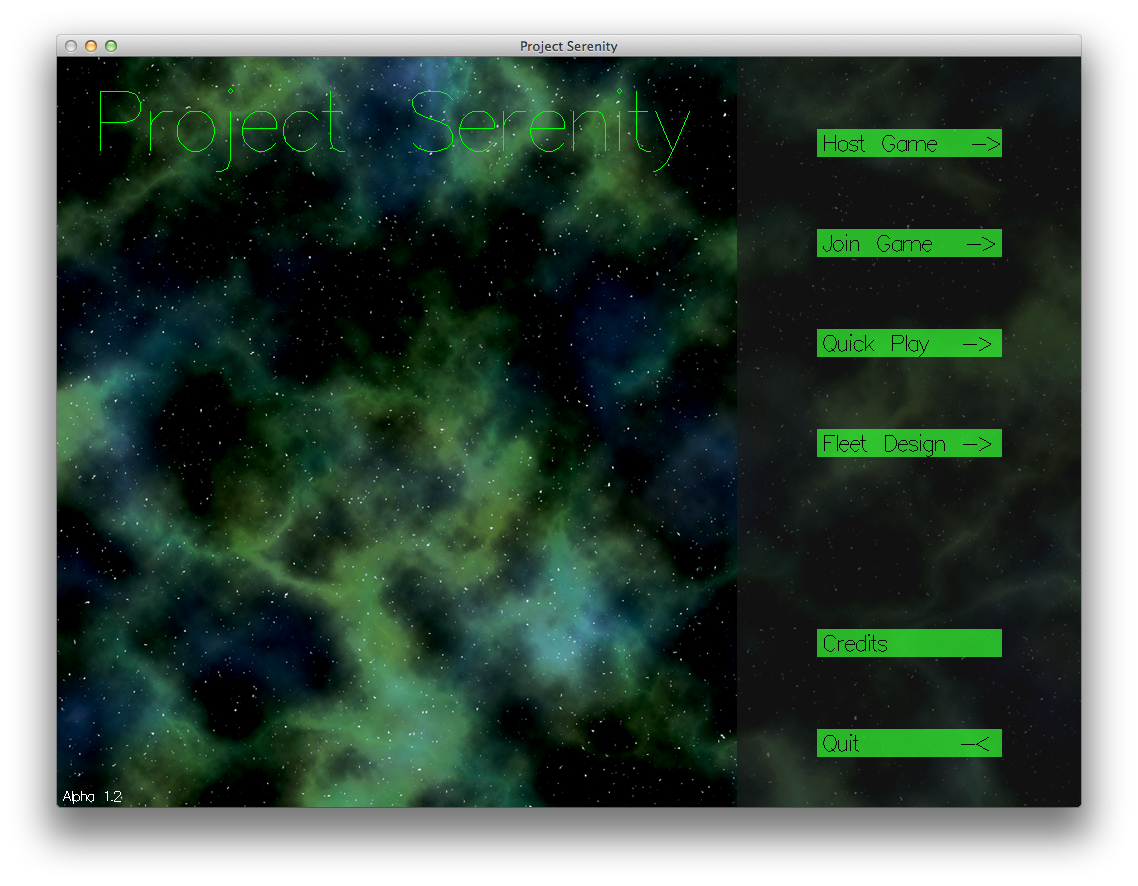
\includegraphics[width=15.5cm]{res/serenityscreens/01-mainmenu}
	\caption[Screenshot of the main menu]{Screenshot of the main menu.}
	\label{fig:mainmenu}
\end{figure*}

\begin{figure*}[p]
	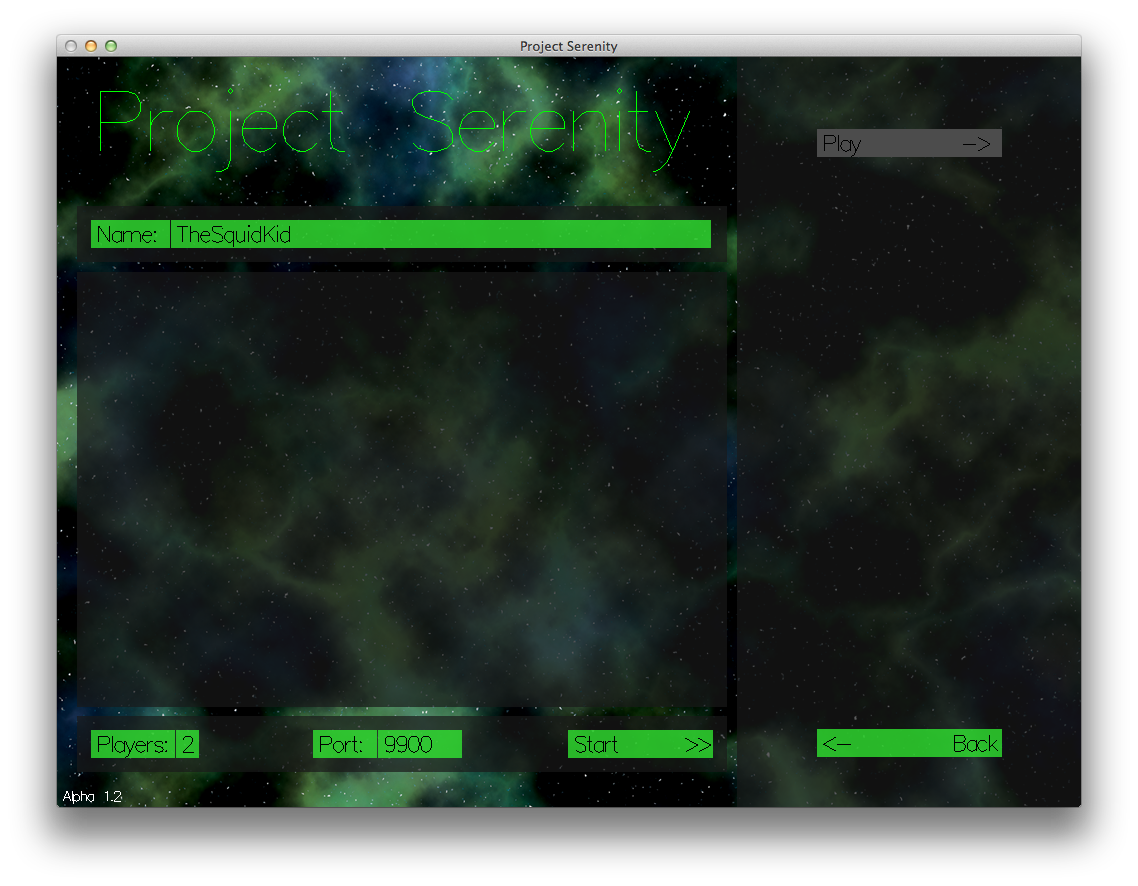
\includegraphics[width=15.5cm]{res/serenityscreens/02-host}
	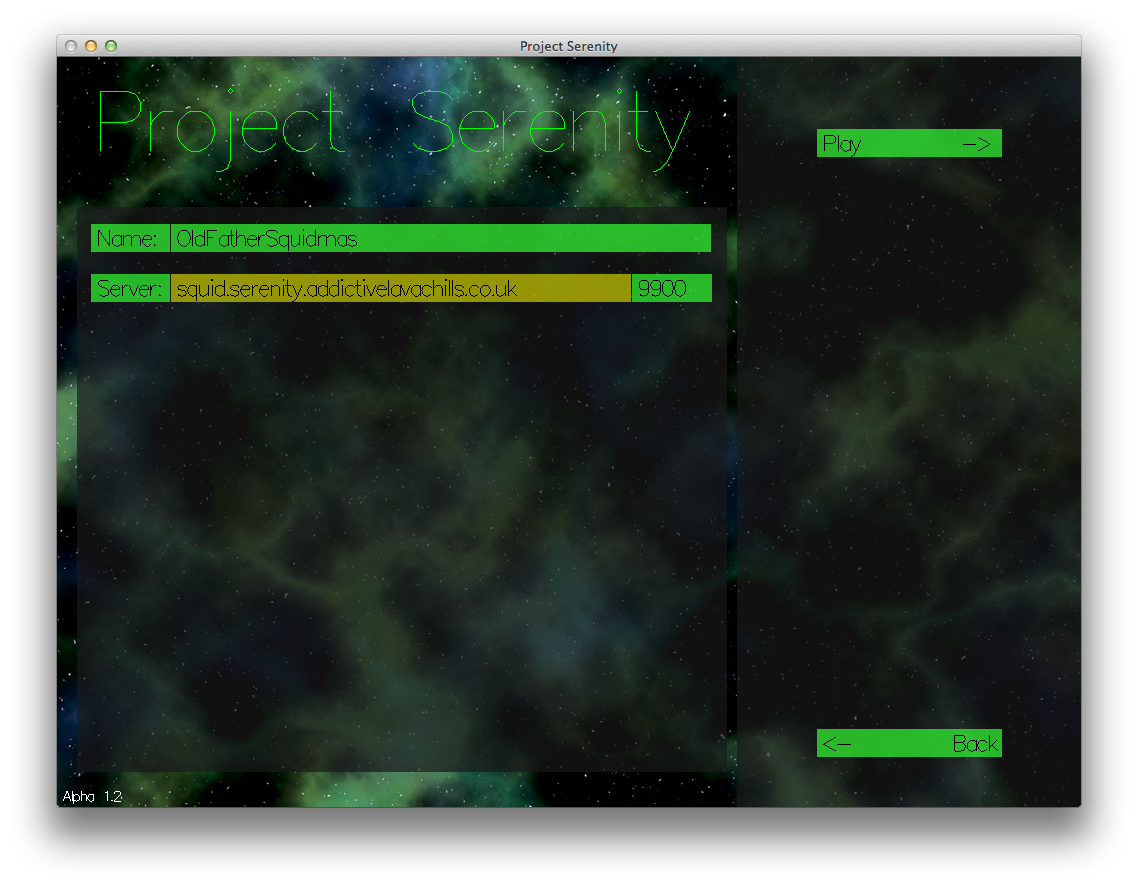
\includegraphics[width=15.5cm]{res/serenityscreens/03-join}
	\caption[Menus for hosting and joining battles]{Screenshot of the menus used to host and join battles.}
	\label{fig:hostjoin}
\end{figure*}

\begin{figure*}[p]
	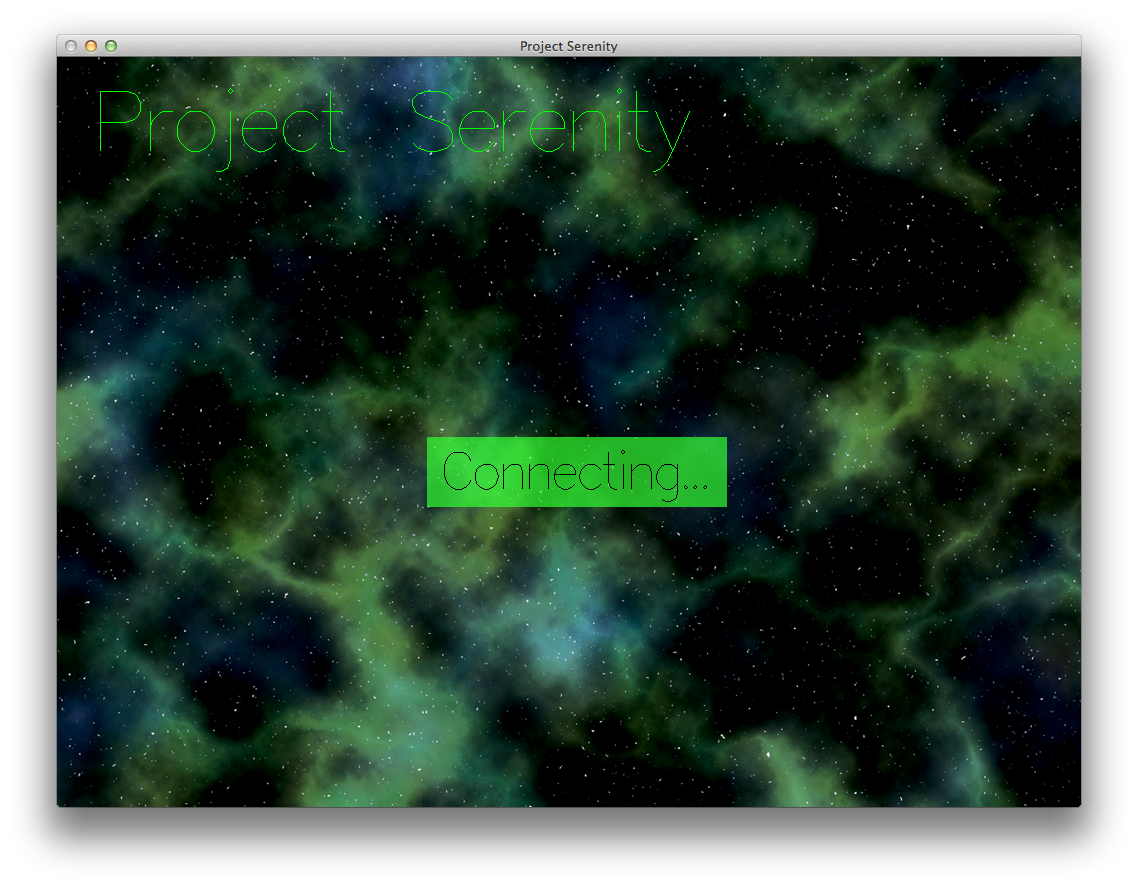
\includegraphics[width=15.5cm]{res/serenityscreens/06-connecting}
	\caption[Screenshot taken as a player connects to a server]{Screenshot taken as a player connects to a server.}
	\label{fig:connecting}
\end{figure*}

\begin{figure*}[p]
	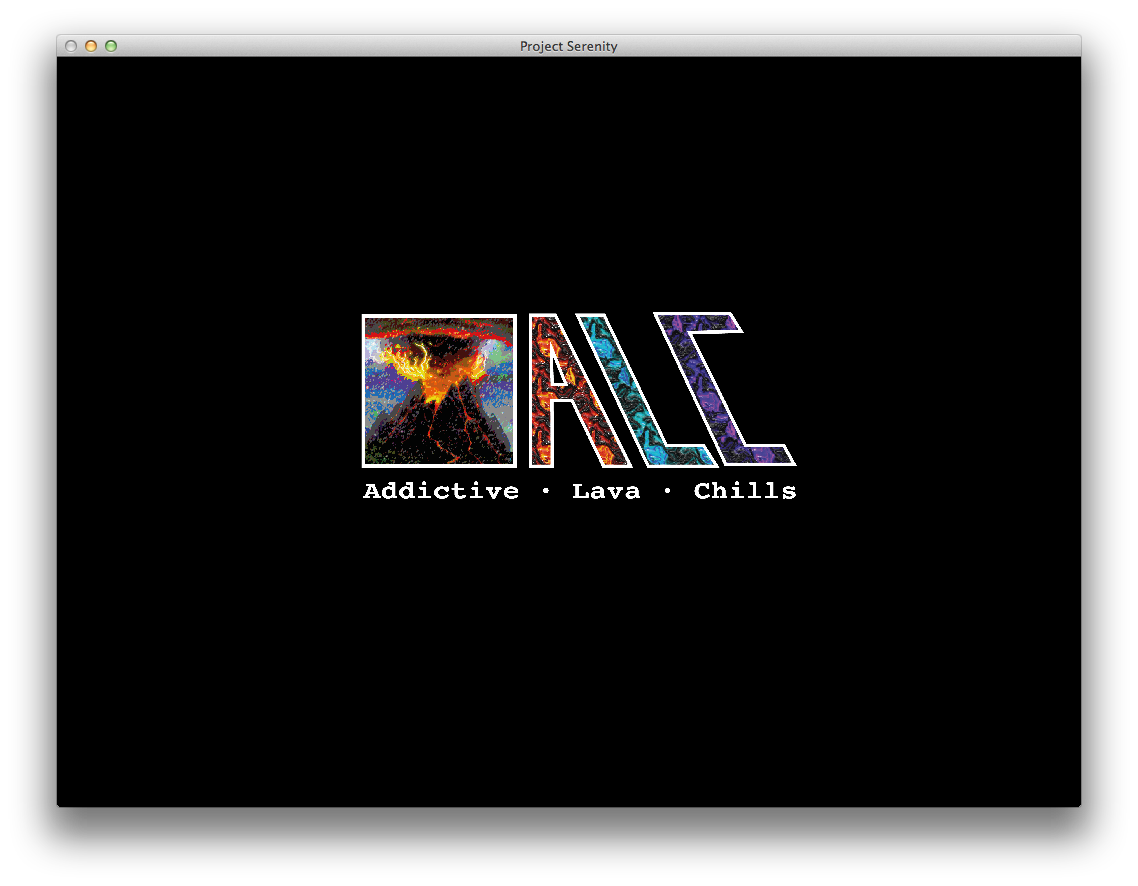
\includegraphics[width=15.5cm]{res/serenityscreens/07-splash1}
	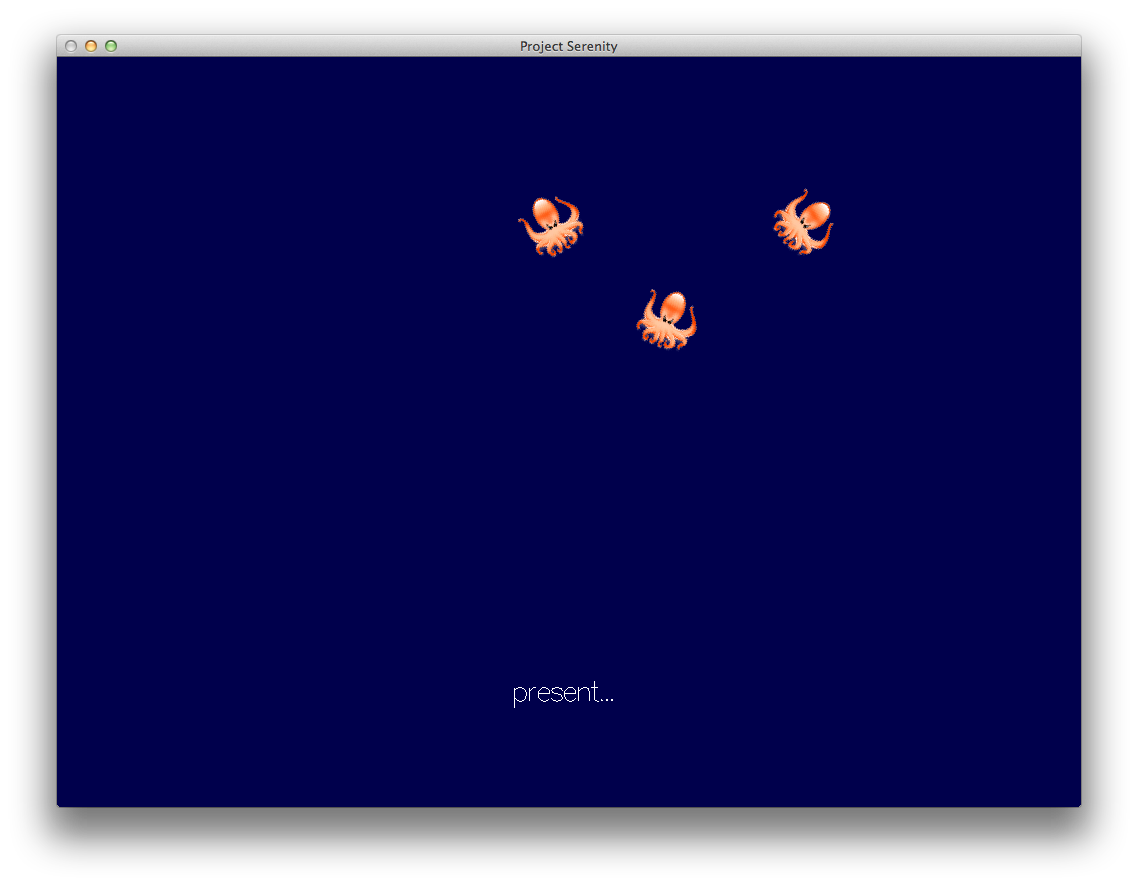
\includegraphics[width=15.5cm]{res/serenityscreens/08-splash2}
	\caption[Splash screens shown on launch]{Screenshot of the splash screens shown when the game is launched.}
	\label{fig:splash}
\end{figure*}

\begin{figure*}[p]
	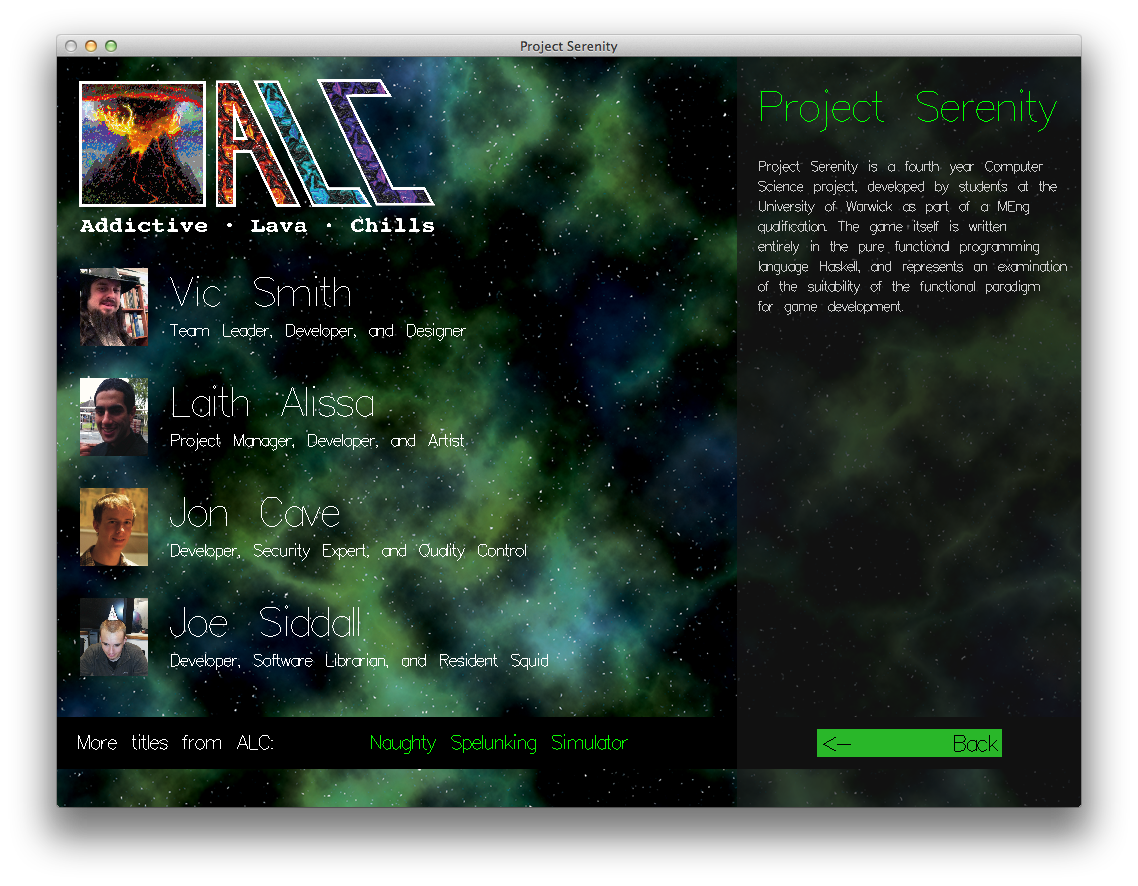
\includegraphics[width=15.5cm]{res/serenityscreens/05-credits}
	\caption[Screenshot of the credits screen]{Screenshot of the credits screen.}
	\label{fig:credits}
\end{figure*}

\clearpage\section{Resources}

\begin{comment}

what are resources

how they effects the game

for each resources:
  - what it's used for

\end{comment}

The resources represent the currency of the game. The player's access to resources can dramatically effect hit chances of winning a battle.

Each resouces has a unique purpose in the game, requiring the player to change strategy dependending on the type and quantity of resources the player has access to.

The three resources are:
\begin{itemize}
\item Fuel
\item Metal
\item Anti-Matter
\end{itemize}

% describe how their are gained (from planets)
Each planet on the map will have a supply of resources. 
The quantity of resources on each planet will vary, but will relate to the planet's type.
When that planet is captured, it will provide a constant trickle of its resources to the player.
For instance if a planet has the following resources:
\begin{description}
\item[Fuel]: 1
\item[Metal]: 2
\item[Anti-Matter]: 0
\end{description}
And is captured by player 1, then every minute, they will receive 2 metal from the planet, and 1 fuel. 
The planet will continue to supply the player with resources until the game ends or another player captures the planet.

% describe how the ship has access to the resources
Each ship will have its own cache of resources on board.
When the ship is near one of it's planets, It will have access to resupply from the player's stockpile. The ship's resource cache will automaticaly refill when near the player's planets. 
Larger class ships have bigger resource caches, and therefore can last longer before needing to resupply (subject to resource consuption).

When a group of ships leaves the safety of its own planets, and starts entering battles, their resource supplies will eventually become empty unless they return to one of their planets. 
If the group of ships continue to battle without resources they will eventually sustain damage to hull and will be more likely to loose the battle.
When a battle takes place within proximately to the player's planet, that player will have the benefit of a constant resupply of resources to the ships in battle. For the other player to win that battle they would need to do so before ship's resources start to dwindle.
This gives the defending player the advantage of endurance, being able to last a battle much longer.


\subsection{Fuel}
When a ship's shields are less than 100\%, Fuel is used by the ship to replenish the ship's shields.
The rate that the ship's shields are regenerated is dependent on the ship class, not the quantity of the ship's fuel cache.
If the ship runs out of fuel, it will stop regenerating its shields.

\subsection{Metal}
When a ship's hull takes damage, the ship is able to repair it on the go with the use of Metal onboard.
The ship will continue to drain it's supply of metal repairing the ship until it has full health again or its metal cache runs out.

\subsection{Anti-Matter}
The rarest of resources, is used as ammunition for a ship's most powerful weapons.
These weapons can only fire if the ship has Anti-Matter on board.
This reason can easilly swap the tide in battle.
\clearpage\section{Planet Capture}
<please insert shizzle here>
\section{Ship Weapons}
% TODO all
% talk about the ships firing arc
% ship weapons(different types of weapons, differences, firing arcs, ranges), do we have more than lasers to talk about?, target targeting)



\section{Modelling the Game}
\label{sec:model}

% what this section talks about
%   - graph of objects and relations
%   - what each model object represents and is
%   - difficulties developing the model
%   - model: sector, game, entity, ship, plan, goal, ship action, ship class, ship configuration, weapon, system, weapon slot, system slot, fleet, Formation, client state
% what is a game model
% early on
% 

The model that makes up the game consists of the internal representation of the various game entities, such as ships and planets, as well as the business logic that is used to manage and control them and the relationships between them. During the alpha phase, this model was rather simple as it only existed to store the locations of the entities. As development progressed, it grew in complexity and feature completeness. Currently there are two sets of models: one for the fleets of ships, and the other for the map of planets and spacelanes.\sidenote{Spacelanes are connections between some planets that allow ships travelling along or nearby them to move more quickly. See Section~\ref{sec:pathfinding} for details.} This section will describe and discuss these models and the reasonings behind their design.

\subsection{Sectors and Planets}

\begin{margintable}
    \begin{tabular}{p{4em} p{11em}}
    \toprule
    \emph{Field} & \emph{Description} \\
    \midrule

    Name & Sector name \\
    Size & Sector dimensions \\
    Spawn points & List of locations where different players' fleets are spawned \\
    Planets & List of planets in the sector \\
    Spacelanes & List of spacelanes that connect the planets \\

    \bottomrule
    \end{tabular}
    \vspace{1em}
    \caption[Fields of the Sector model]{Fields of the Sector model.}
    \label{tab:sector-fields}
\end{margintable}

The different game maps are known as sectors. A sector models all of the planets in a battle, how they are connected with spacelanes, and where the different spawn points are located.\sidenote{Spawn points are locations where a player's fleets will be created} The actual fields that make up the sector model are shown in Table~\ref{tab:sector-fields}. Sectors have different sizes because it allows the players to customise the play time required for a battle to some degree. Choosing a larger sector will typically result in a longer battle than smaller ones. The specification has a requirement for short battles, but it is good to add some flexibility to allow players the freedom to decide how to enjoy the game. It could have been possible to have static spawn points that are enforced for all sectors, for example spawning players in the corners of the sector so that they are as far apart as possible. However, the actual design has per sector spawn points so that the spawn points can be customised to be as fair as possible relative to the layout of the planets within the sector. This decision was made to make the game as balanced as possible to maximise the enjoyment of all players.

% The sector specifies which planets are includes as well as which planets are connected by space lanes as shown in Figure \ref{fig:model:sectorRelation}

% \begin{marginfigure}
% 	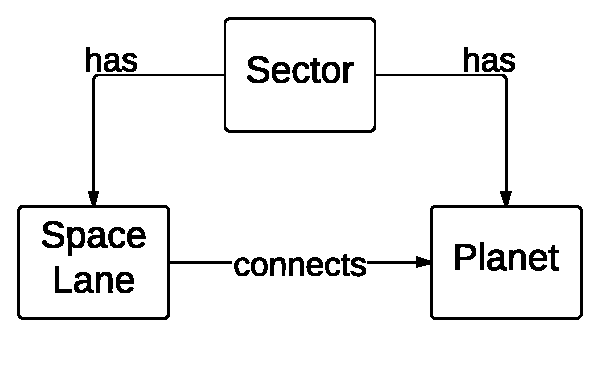
\includegraphics{res/model/sector.pdf}
% 	\caption{relationship between setor, planet, and space lanes}
% 	\label{fig:model:sectorRelation}
% \end{marginfigure}

\begin{margintable}
    \begin{tabular}{p{4em} p{11em}}
    \toprule
    \emph{Field} & \emph{Description} \\
    \midrule
    Name & Planet name \\
    Ecotype & Type of planet, e.g. primordial, ocean, or desert \\
    Location & Location of planet within the sector \\
    Resources & Quantity of resources generated by the planet if captured \\
    Capture status & Current owner of the planet, if any, and by how much they have captured it \\
    \bottomrule
    \end{tabular}
    \vspace{1em}
    \caption[Fields of the Planet model]{Fields of the Planet model.}
    \label{tab:planet-fields}
\end{margintable}

The list of planets that make up the sector are specified using the planetary model. Planets are modelled in such a way as to have a number of different fields that make the planet unique. Table~\ref{tab:planet-fields} gives a breakdown of the properties that comprise the model of a planet. Just like sectors, planets have a name to allow players to easily reference a specific planet instead of having to use location information or a numerical identifier. One of the most interesting pieces of the planetary model is the \emph{ecotype}. The ecotype of a planet specifies the type of ecological system that the planet represents, for example the ocean ecotype is used for planets that are almost entirely covered by water. This ecotype has a big effect on the planet because it determines the quantities of the different resources found in the planet.\sidenote{The use of resources is detailed in Section~\ref{sec:resources}} For example, some ecotypes will have a greater proportion of metal (e.g.\ the metal ecotype). However, the quantity of resources stored by a planet is actually represented by a separate field instead of being statically determined by the ecotype. This was done to make it possible to add some more variety to the different planets. For example, it could be possible to use a random number generator to set the quantities of resources in a planet within the range specified by its ecotype. Currently all resource quantities are specified statically, but this potential enhancement would add some variation to the battles to keep the game interesting for regular players.

% TODO fix margin diagrams, all appearing below the page (invisible)
% \begin{marginfigure}
% 	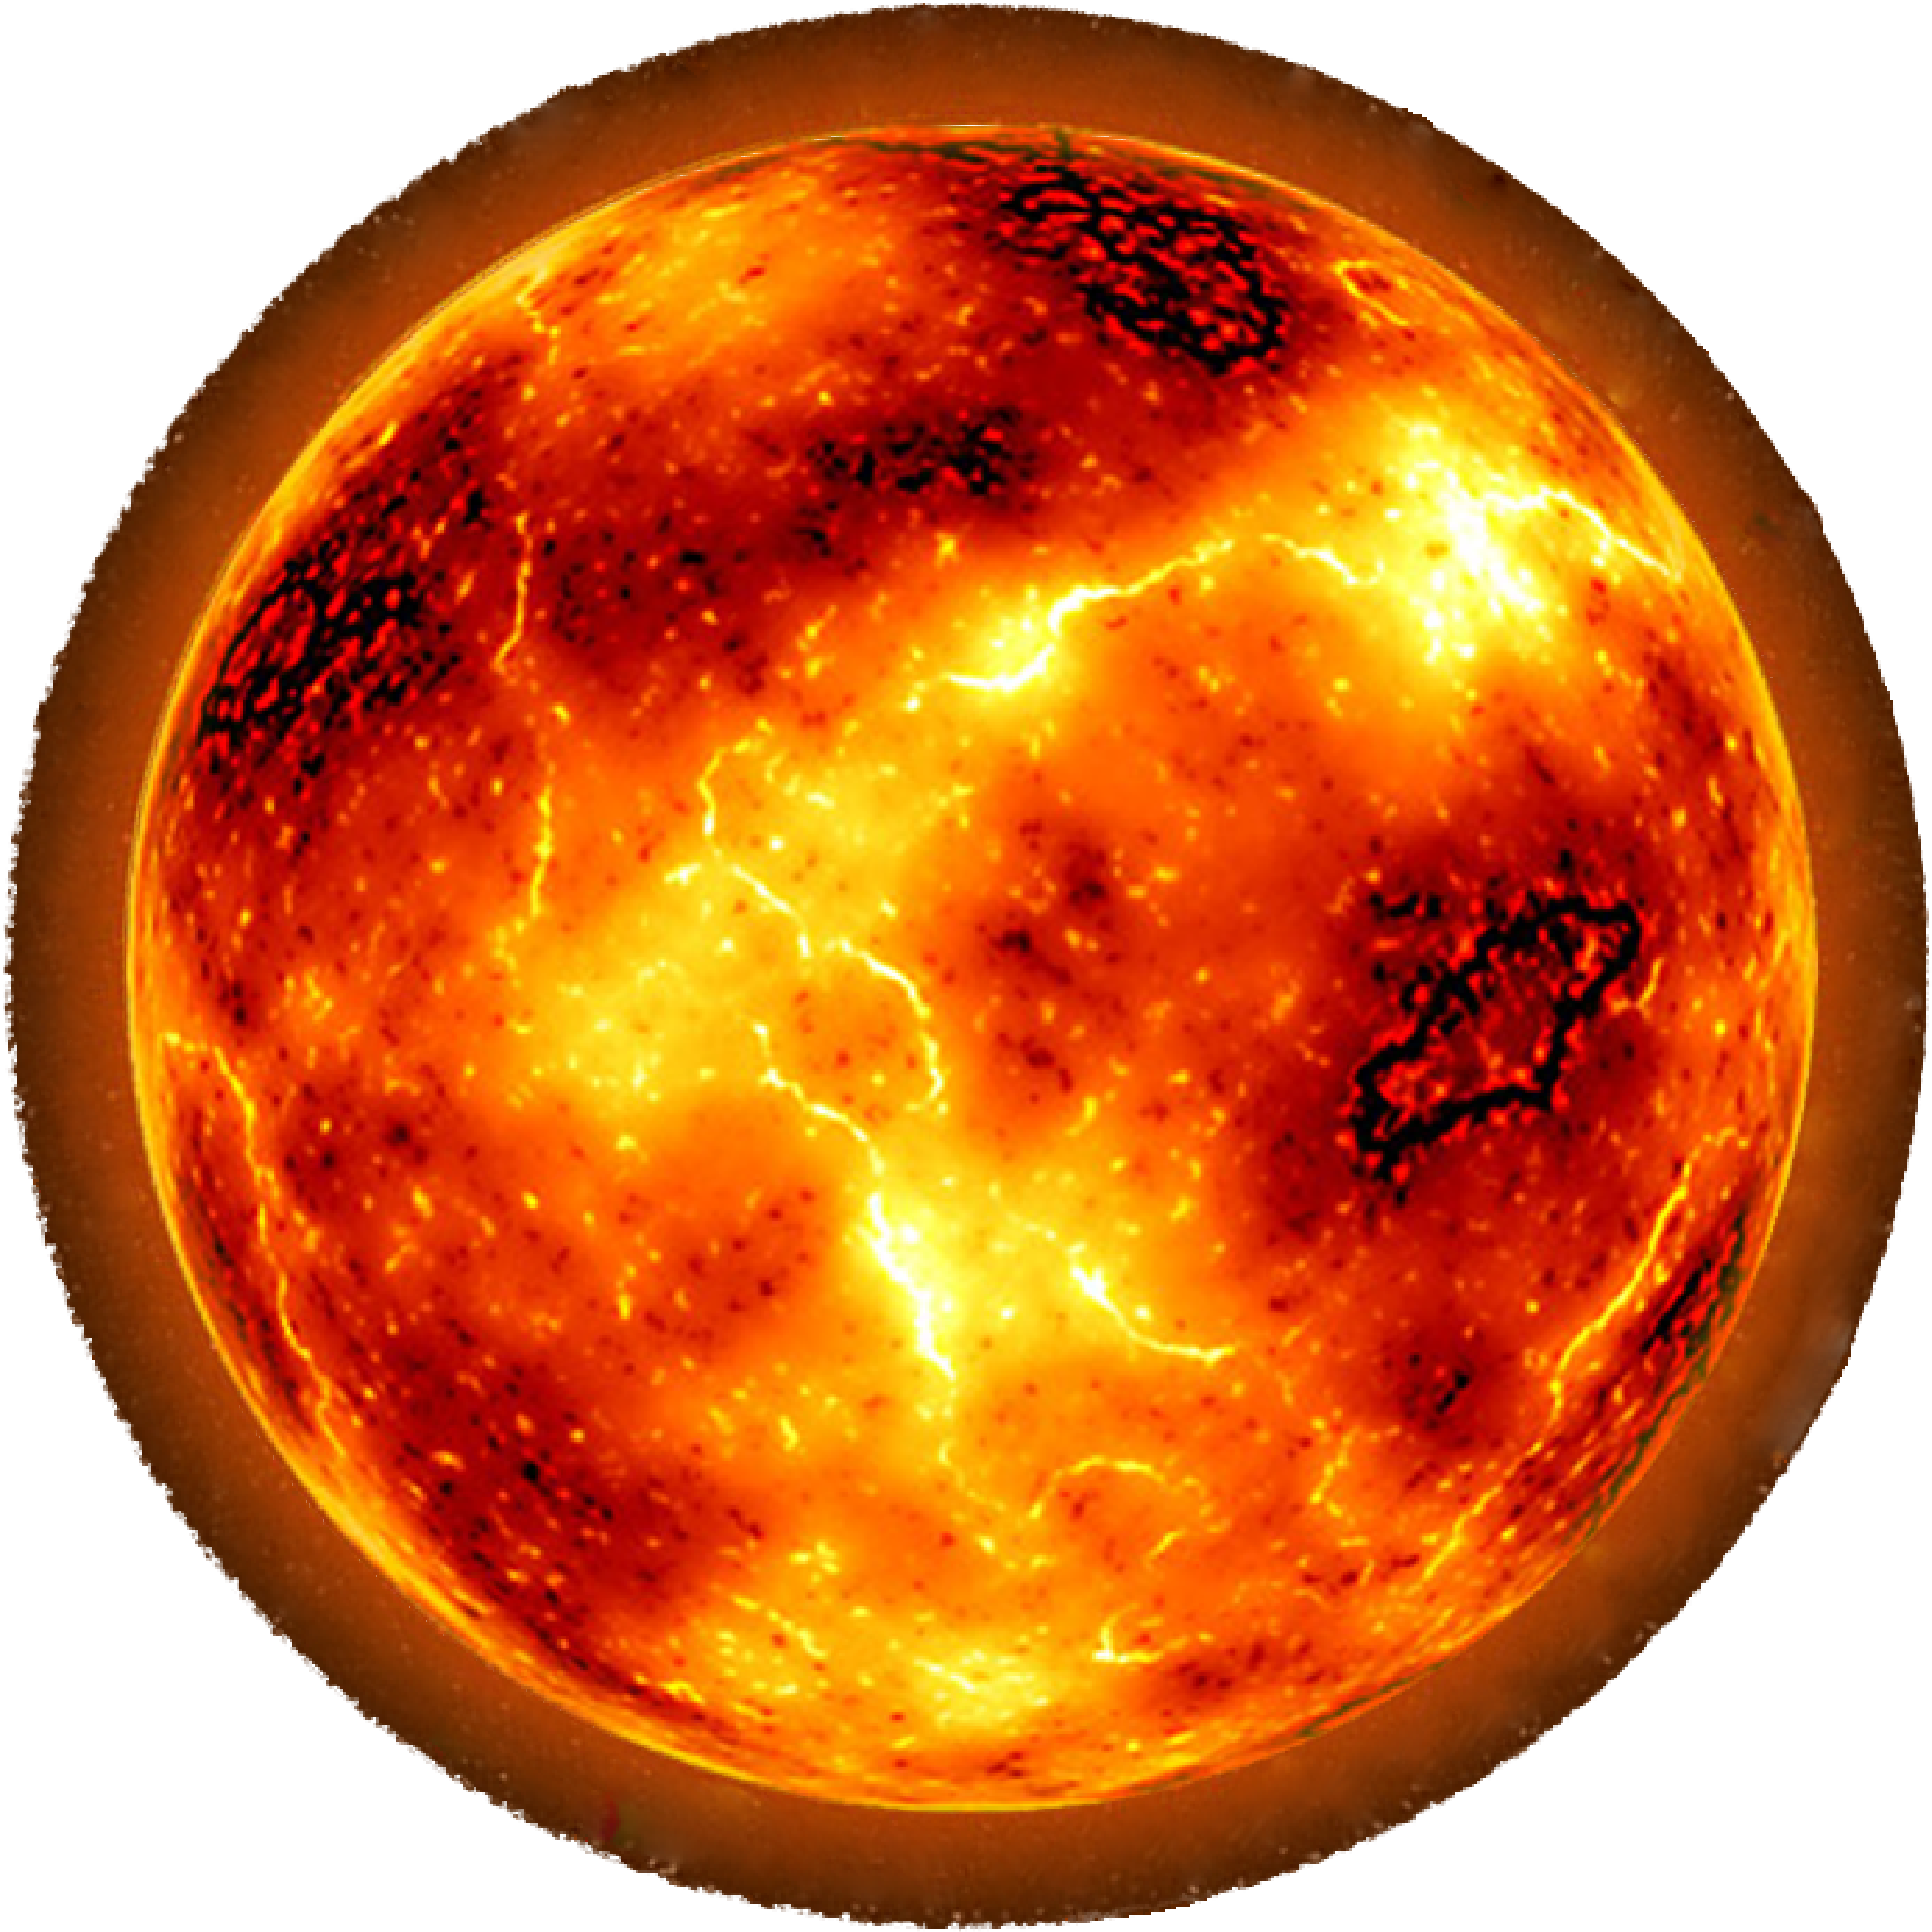
\includegraphics{res/planets/star.png}
% 	\caption{ecotype: star}
% 	\label{fig:model:starPlanet}
% \end{marginfigure}
% 
% \begin{marginfigure}
% 	
\includegraphics{res/planets/OceanPlanet.png}
% 	\caption{ecotype: ocean}
% 	\label{fig:model:oceanPlanet}
% \end{marginfigure}
% 
% \begin{marginfigure}
% 	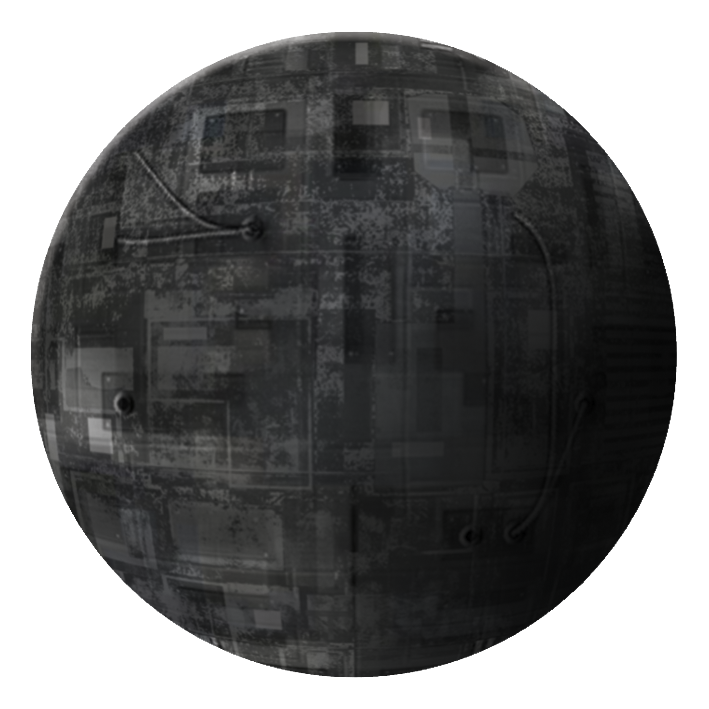
\includegraphics{res/planets/metal-planet.png}
% 	\caption{ecotype: metal}
% 	\label{fig:model:metalPlanet}
% \end{marginfigure}

\subsection{Ships, Classes and Configurations}

\begin{margintable}
    \begin{tabular}{p{4em} p{11em}}
    \toprule
    \emph{Field} & \emph{Description} \\
    \midrule
    Location & Current location of the ship within the sector \\
    Direction & The direction the ship is facing \\
    Damage & How much damage the ship has taken \\
    Order & Current order for the ship \\
    Goal & Current goal the ship is trying to achieve \\
    Plan & Current plan to execute in pursuit of the goal \\
    Targets & List of enemy ships that the ship is attacking \\
    Config. & Class of ship and its customisations \\
    \bottomrule
    \end{tabular}
    \vspace{1em}
    \caption[Fields of the Ship model]{Fields of the Ship model.}
    \label{tab:ship-fields}
\end{margintable}

The second set of models deal with the fleets of ships that are controlled by each player. A fleet is simply a list of ships which a client sends to the server having chosen which ships to include and having made their customisations to these ships. The representation of a ship is actually broken down into a generic ship model and its specific configuration. The general ship model contains the configuration as well as the attributes that are updated during game play, such as the ship's orders and plans, and its current location and direction. The full list of fields for this model is shown in Table~\ref{tab:ship-fields}. The use of location, direction, and damage should hopefully be obvious. They can be updated every tick by the server's main loop as the ship moves around the sector and engages with the enemy. Orders, goals, and plans are used by the artificial intelligence that controls the ships, see Section~\ref{sec:ai} for more details. The list of targets that a ship is currently attacking is also controlled by the artificial intelligence. The most interesting part of the ship is its configuration which specifies what ship class it is and the customisations that have been applied by the user.

The ship configuration contains the chosen ship class along with the lists of weapons and support systems that the player selected to add to the ship. The ship class represents the type, or blueprint, of ship specifying the basic statistics of the ship. The set of statistics defined by the class is: speed, hull health, shield health, details of each of the weapon slots, details of the support system slots, and the cost of the ship. These statistics are used by the simulation code in the server to determine how the ship moves, how much more damage it can sustain before being destroyed, how much damage it does to the enemy ships it is attacking, and so on. A player is able to select the set of ship classes that they wish to include in their fleet, but they are restricted by a fixed budget. There are three ship classes that come with the game by default: corvette, destroyer, and dreadnought. The corvette is the smallest and quickest ship that can only be given one weapon. The destroyer is of middling strength and speed, it allows for five weapons to be added. Finally, the dreadnought is the largest and slowest of the three, but it packs the largest punch by supporting up to nine weapons.

This layered model approach to representing the ships was used to separate the different types of data that have to be stored. The ship model deals with the dynamic data that is updated during gameplay, the ship class is concerned with the static statistics that define the ships behaviour, and the configuration stores the user's customisations. This is useful because it allows a more efficient method of storing custom fleets on disk. Only the list of ship configurations needs to be kept since the class data is the same for all ships of the same type so can be loaded at run time and the rest of the ship data is only relevant during a battle.

% \begin{marginfigure}
% 	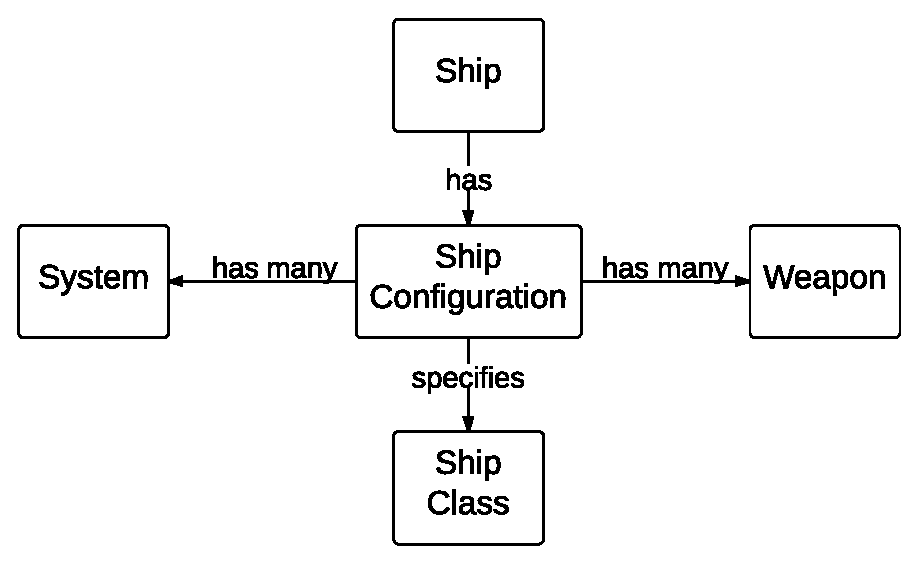
\includegraphics{res/model/ship.pdf}
% 	\caption{ship layout}
% 	\label{fig:model:shipRelation}
% \end{marginfigure}

\subsection{Weapons and Support Systems}

% TODO all
% talk about the ships firing arc
% ship weapons(different types of weapons, differences, firing arcs, ranges), do we have more than lasers to talk about?, target targeting)

Before a battle is started, a user is able to customise the ships that make up their fleet. They do this by first selecting the types of ships to use and then filling the pluggable slots with extra parts. There are two types of part: weapons and support systems. Weapon slots are arranged in three different locations around the ship. Side weapons are used to fire to the port and starboard of the ship. The front weapon slot, if present on a ship, can hold a weapon which fires on the front firing arc. Finally, there are turret slots that allow a weapon to shoot in all directions apart from backwards. Support system slots are used to hold extra internal systems to enhance the ships abilities, such as shield boosting or cloaking devices. This ability to add different parts to a ship was one of the functional requirements laid out in the project specification, so the availability of some parts to use is of great importance to the game.

The ship configuration holds two lists that describe the weapons and support systems that have been added to the ship by the user. These lists represent the filling of the pluggable slots that are part of a ship. The game comes with two types of weapons pre-defined. Lasers are relatively short-range weapons that inflict a medium amount of damage on enemy ships, and rockets are much longer range weapons that cause a great deal of damage. Just like ships, the weapon stats are stored in a model. The weapon model holds the range and damage information of each weapon type so that it can be referenced by the server to determine which ships are eligible for targeting and how much damage they should receive.

Currently, the support system model is much less developed than the weapons. So, at this time, there are no available support systems that can be used to add performance to a ship.

\subsection{Defining Model Instances}

All of the different ship, weapon, and system types that have been discussed so far are not actually hardcoded into source code of the game. Instead they are defined in external configuration files that are loaded by the game code at run time --- therefore, these types are collectively known as addons in the parlance of the game. This route was chosen because it would allow easy modification of the attributes of these addons without having to recompile the source code. So, players who are not able to program still have the option of changing some of the statistics to customise gameplay. It also possible for players to add their own custom addons to enhance the game with more options for fleet customisation. Allowing the game to be modified in this way is hugely popular in the gaming community. For example, \emph{Counter-Strike} began life as a community built mod of the game \emph{Half-Life} before becoming the most popular game in the world.\cite{lambdageneration2012}

\begin{marginfigure}
    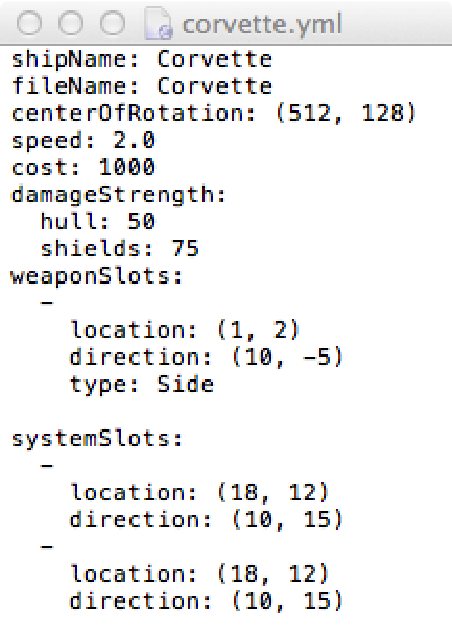
\includegraphics{res/configuration/corvetteYaml.pdf}
    \caption[Example of a YAML configuration file]{Example of a YAML configuration file.}
    \label{fig:corvette-yaml}
\end{marginfigure}

The addon definitions are stored in YAML files in the resources directory. YAML was chosen as the file format due to its focus on human readability. Other serialisation formats, such as XML and JSON, were considered, but were discarded in favour of the combination of brevity and readability afforded by YAML. When the game is launched, the resources directory is scanned for YAML configuration files and the data is loaded into memory. Adding new instances of models only requires adding a new YAML file to the appropriate directory, and configuring existing ones is as simple as editing a text file. Figure~\ref{fig:corvette-yaml} shows the corvette ship type defined in YAML.

\clearpage\section{Artificial Intelligence: Orders, Goals, and Plans}
\label{sec:ai}

A sophisticated artificial intelligence (AI) system was highlighted as one of the major
functional requirements for the project. The plan was to use the AI to take high
level orders from the player and convert them into a detailed plan for individual
ships to execute. In this way the player would direct the overall strategy of their
fleet, but without actually captaining the individual ships. This would reduce the
amount of micromanagement a player has to undertake and increase the sense of realism
--- the admiral of a real fleet is unable to directly control individual ships under
their command. This plan for a high level AI was seen as one of the larger challenges
that the project would face.

Artificial intelligence can often be a make-or-break factor in determining the success of
a game.\citepage{rabin2002}{page 3} Without a convincing intelligence system, a game can
quickly become infuriating to play. This is because a human player expects any computer
controlled components to behave sensibly. In some cases well known algorithms exist that
enable `intelligent' behaviour to be implemented relatively easily, for example the use
of the A* search algorithm for pathfinding. However, higher level intelligence systems
are much more challenging. A system capable of creating and executing quality plans
from abstract orders is going to be one of the hardest components to implement.

As well as providing an entertaining experience an AI system must also be efficient.
There cannot be large delays between the user giving an order and it being carried
out. Any planning algorithms have to run quickly otherwise the lag in feedback will
detract from the realism of the game. An inefficient AI system could also stop the game
from running smoothly --- which is of great importance for a real-time strategy game.
This would lead to a poor user experience causing people to stop playing the game.
For these reasons, careful thought was put into designing a system that could fulfill
the important requirements for a successful AI system.

The AI framework that was implemented in Project Serenity is based on a planning
hierarchy. At highest level are orders, such as move to a given location or capture
the specified planet. These orders are under the control of the player, but it is
the job of the AI system to plan a series of actions to achieve them. The first step
is to convert the order into a goal. There is mostly a one-to-one mapping between
orders and goals, for example "OrderMove" maps to "GoalBeAt", however this layer of
abstraction allows the AI to choose unrelated goals if the current order is impossible
or would result in the needless loss of a ship. The goal is then decomposed into a
plan which is a series of actions that are performed to complete the current goal
(and hopefully fulfill the current order too).

The current planning cycle for a ship is as follows:

\vspace{-0.5em}
\begin{listing}{list:planning}{Planning cycle pseudocode}{Pseudocode for the AI framework's planning cycle.}{}
\end{listing}\vspace{-1.5em}

\begin{tabbing}
{\bf if} the current plan is empty {\bf then} \\
\quad{\bf if} the current order is complete {\bf then} \\
\quad\quad Reset the ship's order to "OrderNone" \\
\quad\bf else \\
\quad\quad $g \leftarrow$ create goal from the current order \\
\quad\quad $p \leftarrow$ create a plan from the new goal, $g$ \\
\quad\quad Update the ship's goal and plan with $g$ and $p$ \\
\quad\bf fi \\
\bf else \\
\quad{\bf if} the first action in the current plan is complete {\bf then} \\
\quad\quad Remove the action from the head of the ship's plan \\
\quad\bf else \\
\quad\quad Perform the action at the head of the ship's plan \\
\quad\bf fi \\
\bf fi
\end{tabbing}
\noindent
This planning cycle runs every server tick so that all ships in the game can
continuously formulate and update their goals and plans.

An improvement to the planning cycle would be to add in periodic replanning steps.
This would allow a ship to change its plan if the world around it changes, for example
to disregard an order to capture a planet if it is guarded by multiple enemy ships
and there is no friendly support in the area. In the current implementation this is
done on a bit of an ad-hoc basis instead of being formalised into the planning loop.
For example, the code that implements the action to move to another ship will check
if the target ship is still near to its location when the plan was originally formulated.
If the target ship has moved too far then the current plan is scrapped so that a new
plan can be constructed.

\subsection{Targeting Enemy Ships}

As well as constructing a planning framework for executing player given orders,
it was necessary to build some systems to carry out intelligent actions outside
of the usual planning loop. One such example is that of targeting enemy ships to
attack. As a ship moves about the sector it will fire upon any enemy ship that
it encounters. However, if there are multiple ships in the vicinity then it is
necessary to select which to target as it may not be possible to attack all of
them at once. A clever targeting system had to be devised to solve this problem
in an effective manner.

The first step is to generate a list of all potential enemy targets. This is a list
of all enemy ships that are in range of any of the ship's weapons. A list of
enemy ships to attack is selected for each weapon by taking the enemy ships that
would be attacked by the least number of other weapons as well. This method of
target selection means that a ship will spread its attacks out to hit as many
enemy ships as possible.

This pattern of list generation and selection fits the one described by John Hughes
very well.\cite{hughes1989whyfp} This is one of the reasons why the Project Serenity
team found Haskell to be highly adept for programming AI algorithms. The separation
between the potential target list generation and the selection from the list also means
that it would be very simple to modify the selection strategy. For example, a
possible enhancement to the game would be to allow players to configure a targeting
strategy for their fleet which would focus attacks on the weakest enemies.

%% todo: Fix 3.6 captions when jon and vic are done

\clearpage\section{Ships, Spacelanes, and Path Finding}
\label{sec:pathfinding}

The specification made it clear --- by the way weapons and navigation between planets was to be structured --- that ship motion needed to be relatively detailed. It is no use having a weapon that can be only used in one arc if ships could instantly pivot on the spot. Instead it was desired for ships to move as large objects with a great deal of momentum, with large turning circles and ponderous movements. However it would be undesirable for the motion of ships to be too realistic, as it would make the game needlessly difficult and confusing. A real object undergoing acceleration in space could of course, accelerate essentially indefinitely (until it was nearing the speed of light) but would need to take an equal amount of time to decelerate to stop again.

\begin{marginfigure}
	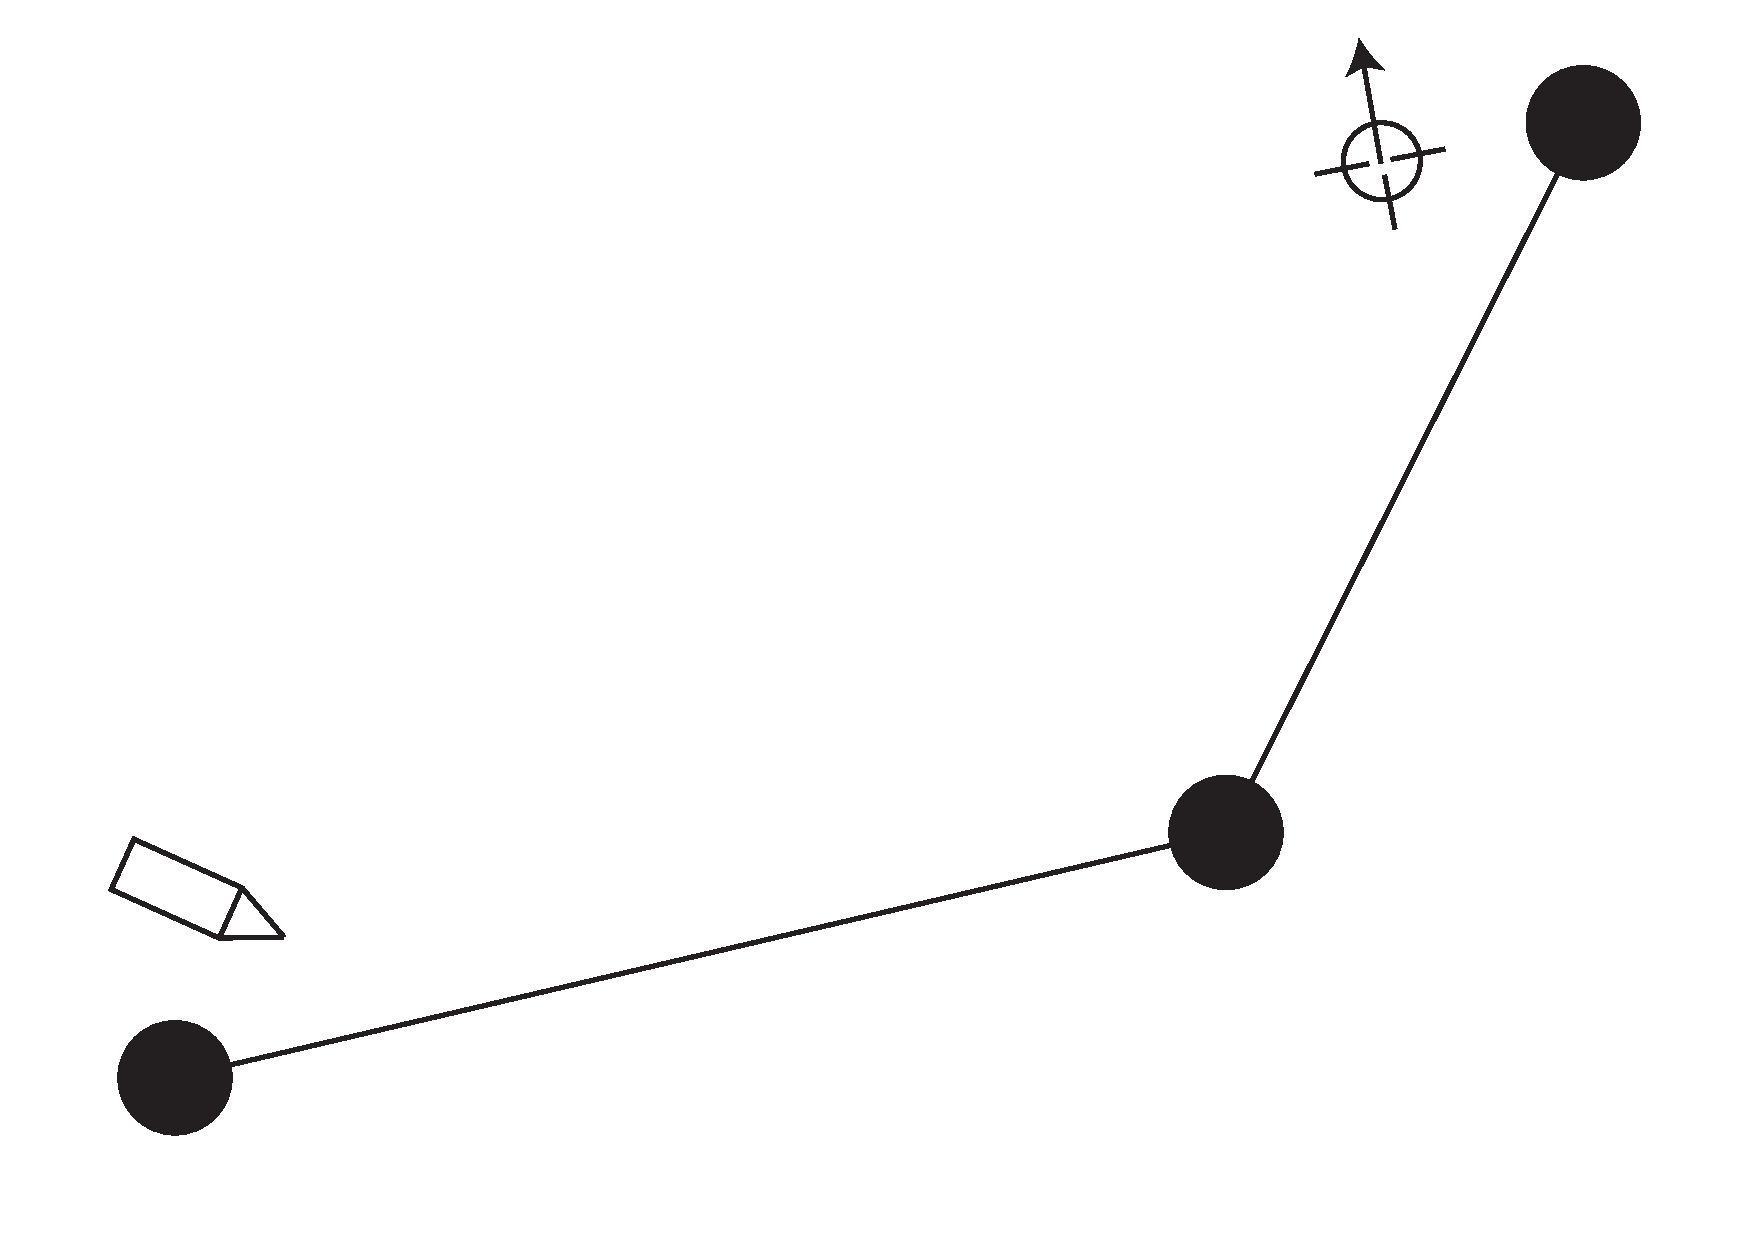
\includegraphics[width=20em]{res/pathfinding/spacelanes}
	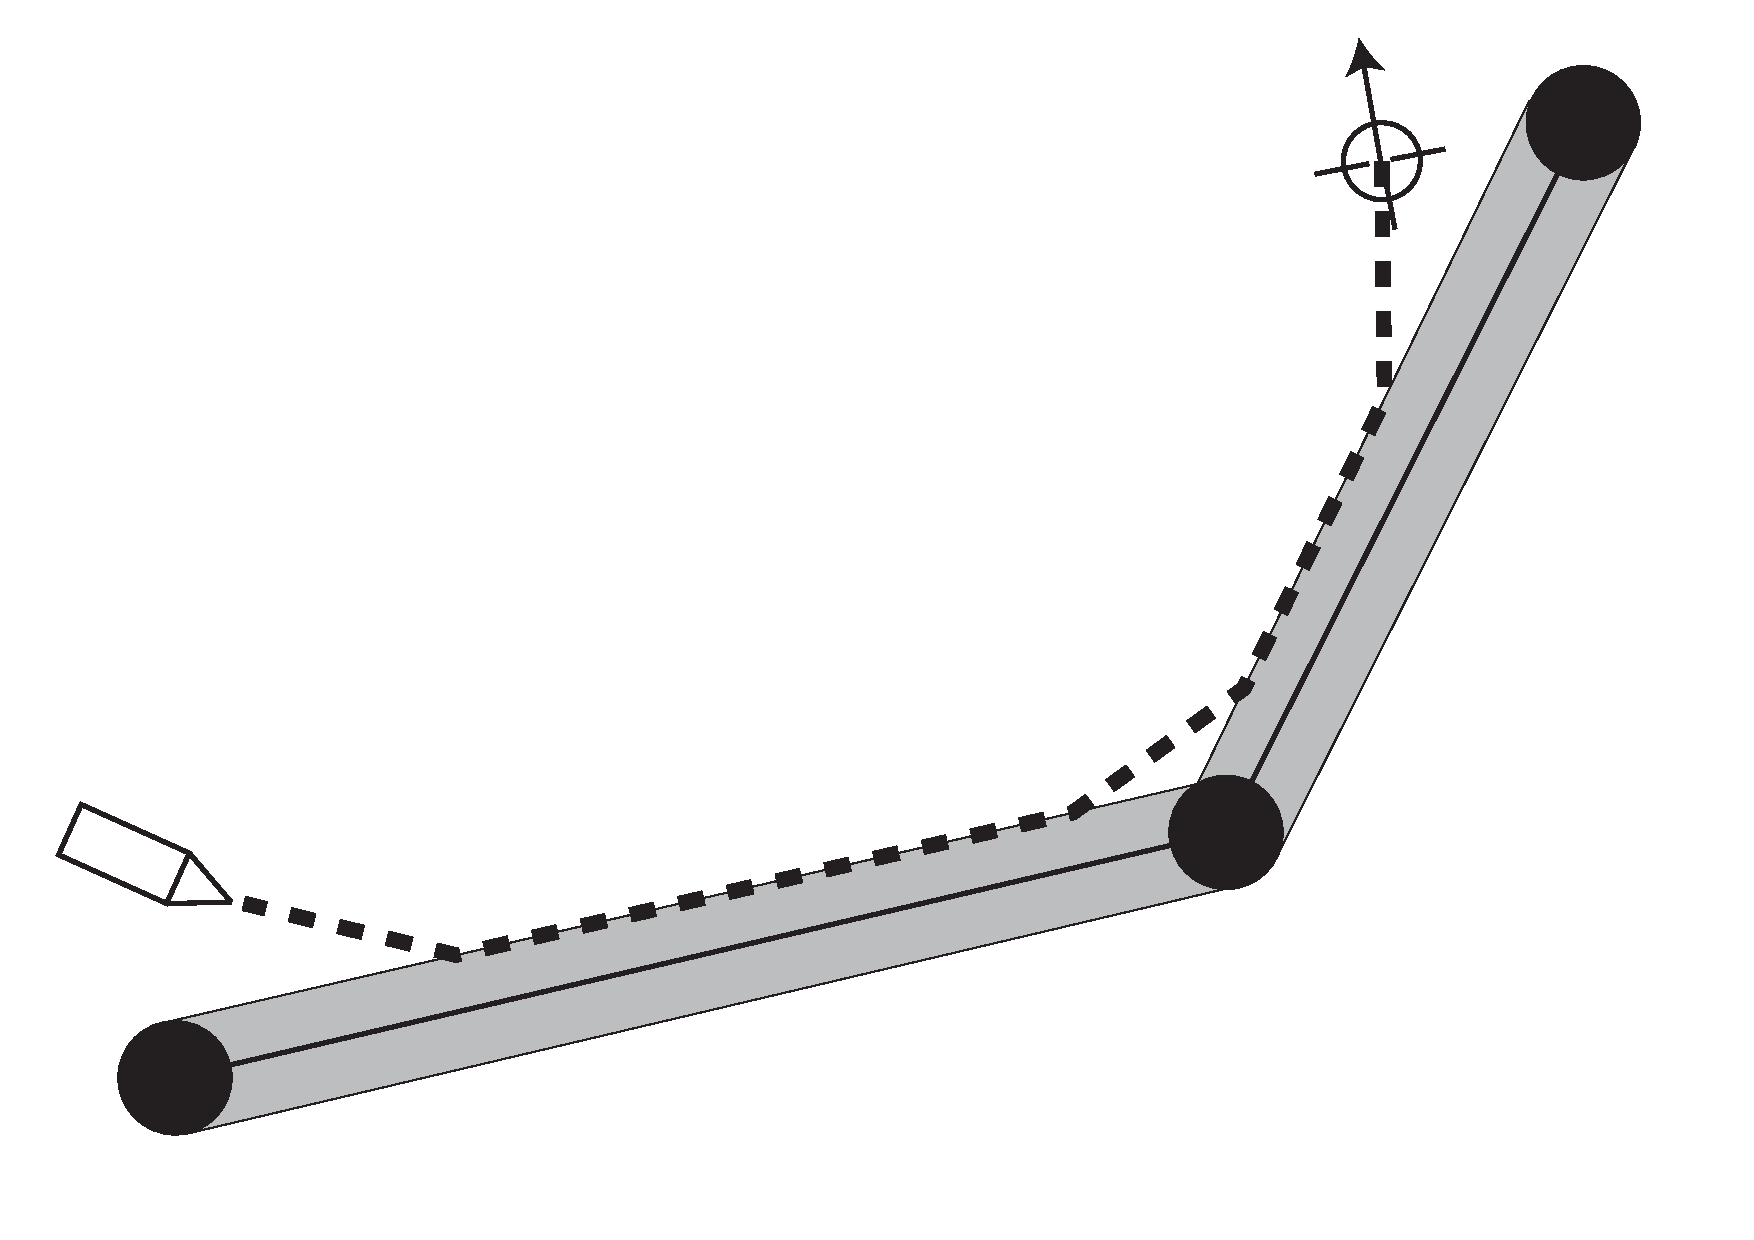
\includegraphics[width=20em]{res/pathfinding/spacelanes_ray}
	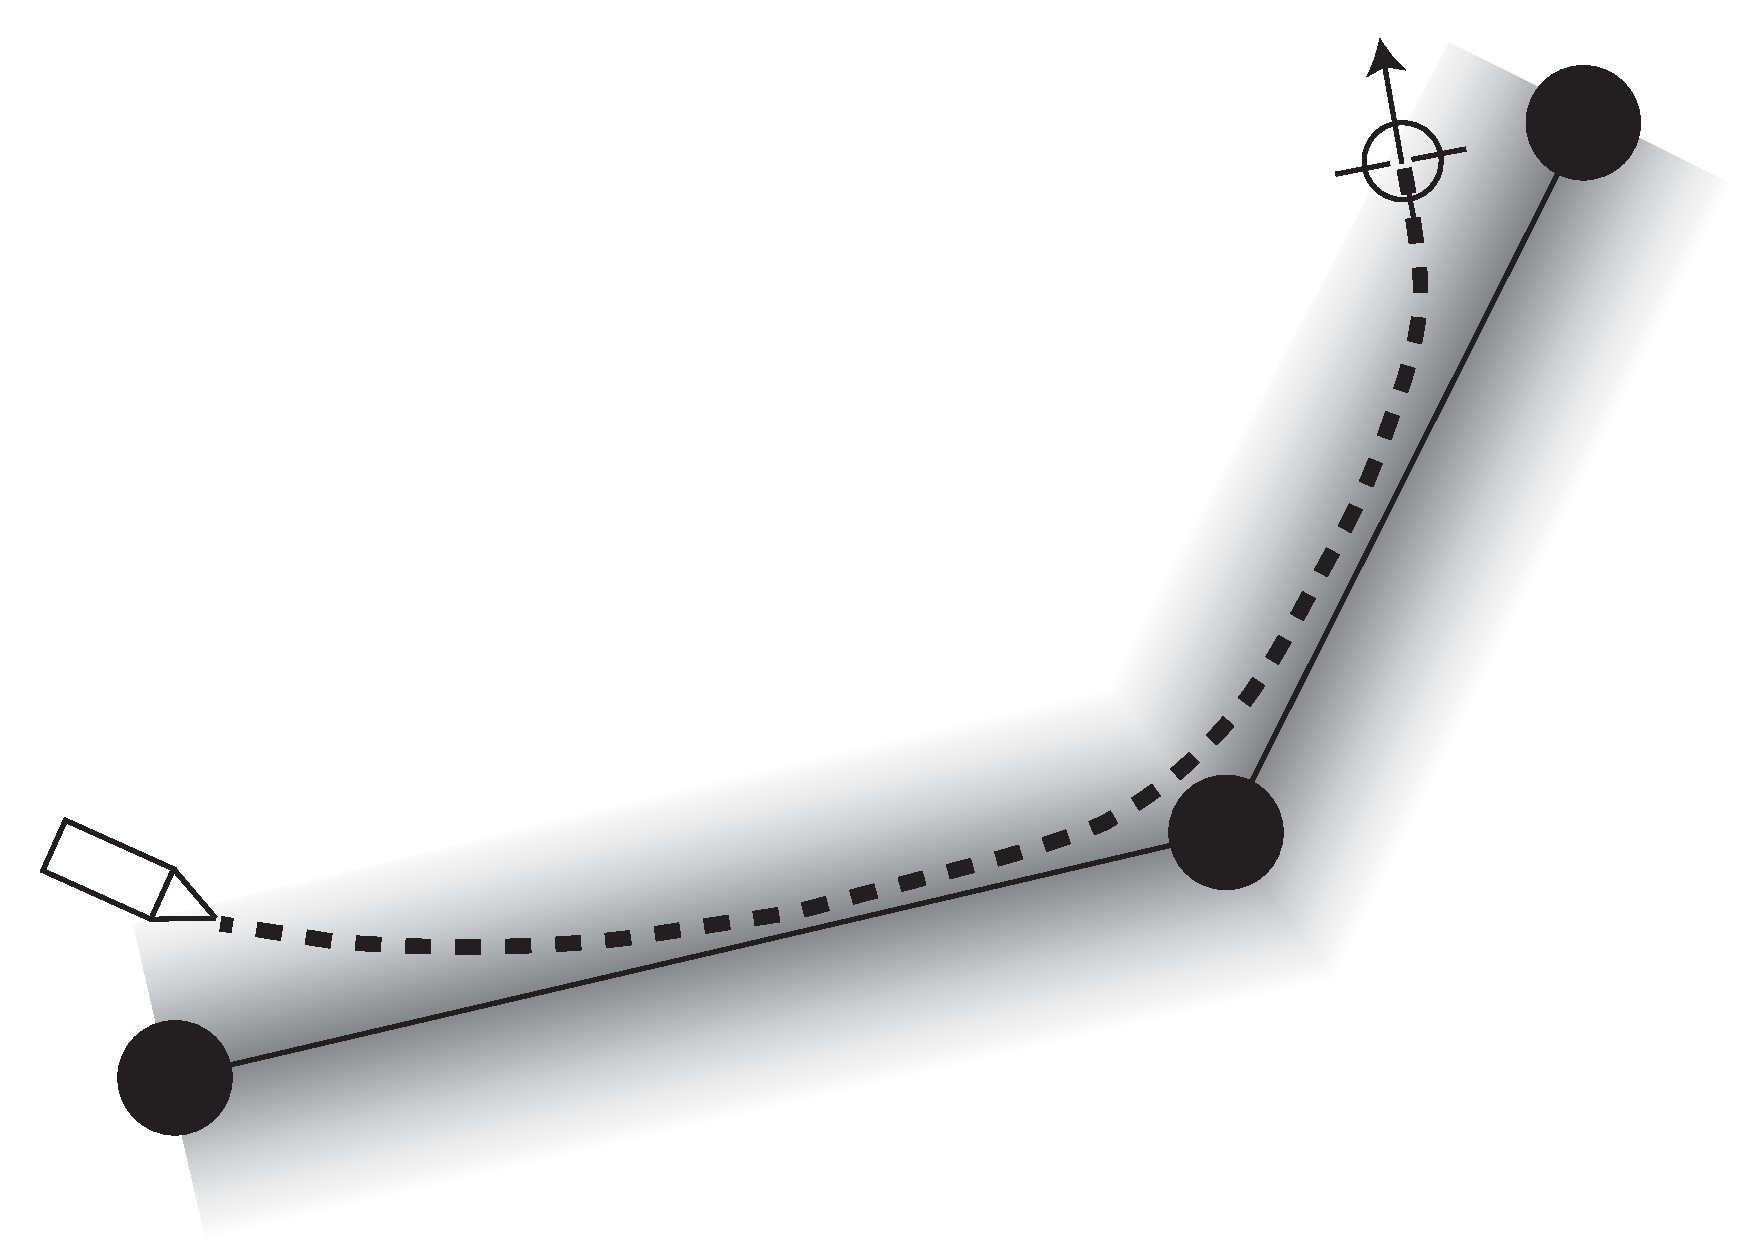
\includegraphics[width=20em]{res/pathfinding/spacelanes_field}
	\caption[Illustrations of different models for a path between current location and target utilising a spacelane]{Illustrations of different models for a path between current location and target utilising a spacelane.}
	\label{fig:spacelanes}
\end{marginfigure}

Intimately related to these questions is the precise nature of the \emph{spacelane} mechanics. Spacelanes between planets were introduced into the game in order for the otherwise empty space between planets to have some strategic topology, the idea being that the spacelanes can be traversed much more quickly than empty space. and so control of the lanes are vital to a successful strategy. Many different models were discussed for this mechanic during design meetings, both from the point of view of the in universe explanation, and the precise way in which the game would implement it. Initial ideas on the physical mechanism of the spacelane was that they conferred an additional optional acceleration: i.e. that if a ship is approximate to a lane it could opt to undergo greater acceleration than a ship far from a lane. But as mentioned, accurately modelling acceleration in space is somewhat contrary to the gameplay aspirations of the design. 

A simpler mechanic for ships that was considered to be more suitable, is for them to have a top speed that they could reach relatively quickly; but for them to still have large turning circles. This makes their motion more similar to naval ships engaged in warfare. The interpretation of the spacelane in this model cannot be simply a gain in acceleration as this confers little benefit. Instead it is clear that the spacelane must confer an addition to top speed. A possible physical interpretation of these behaviours is that the ships are moving in some kind of ether with friction, and so will reach a terminal velocity. The spacelane is then an area with an artificially induced lower density of ether.

Another fundamental question about the nature of the spacelane is whether its effects are immediately felt at full strength at a certain distance from it, or whether they fall off related to distance. the former is most definitely simpler, but the latter feels more natural as a mechanism. Figure~\ref{fig:spacelanes} shows the difference in the shortest paths that these approaches may generate, discounting the additional issue of ship turning.

\subsection{Algorithms for Pathfinding}
% physics hard
% bezier (not trivial)
% flow fields

Physical simulation of a large mass moving and turning in space was the initially preferred implementation method, but it became increasingly clear that this was going to be difficult both from an implementation and a user perspective. And while modelling the spacelane as having a continuous, field like nature, it was not at all clear how this would be achieved. It was decided to instead merely approximate the desired behaviour using bezier curves.

\begin{marginfigure}
	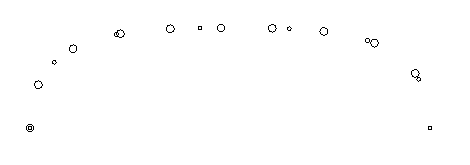
\includegraphics[width=20em]{res/pathfinding/bezier}
	\caption[Bezier path at regular intervals]{Bezier path at regular intervals (small circles) and the same path after having been reparameterisated by arc length (large circles).}
	\label{fig:bezier}
\end{marginfigure}

Over the Christmas break the code for a ship moving between two arbitrary points and headings was developed. Coding bezier paths themselves was not difficult, but moving an object continuously along one at a constant speed was much more complicated than expected. The accurate solution of this problem is called reparameterisation by arc length, and requires a solving a differential equation, but the method eventually used in Serenity was a numerical interpolation. Results are shown in Figure~\ref{fig:bezier}.

\begin{marginfigure}
	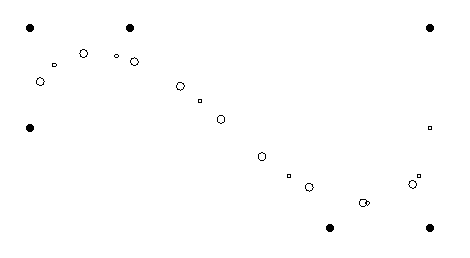
\includegraphics[width=20em]{res/pathfinding/bezierpath}
	\caption[Bezier path at regular intervals]{Bezier path at regular intervals (small circles) and the same path after having been reparameterisated by arc length (large circles).}
	\label{fig:bezierpath}
\end{marginfigure}

Even with the ability to move a ship smoothly along a given path, the selection of the path still required some considerable thought. An example of the control points generated for a move is shown in Figure~\ref{fig:bezierpath}.

\subsection{Applying A* to a Sector}
% what is the problem
% why this is no trivial problem
% Why A*

Applying a pathfinding algorithm to a sector has two stages: generating a graph which represents the sector, and running the algorithm that traverses the graph to find the shortest route to the destination. The algorithm chosen for the second stage is A* because it will always find the optimal solution (assuming the heuristic is admissible) and, if an efficient heuristic is used, then it is very fast too. However, the difficulty of using A* is that it requires a discrete graph to navigate, but the sector is not discrete as ships can move anywhere within it. The planets and spacelanes provide some points of reference, but they do not restrict the movement of the ships. Therefore, it is necessary to build a discrete graph from the sector model during stage one.

Just using the planets as nodes connected by edges of spacelanes does not work since the ships can go into other areas of space not covered by such a graph. Advanced techniques such as constructing a navigation mesh or a waypoint graph do not really apply in this situation since there are no obstacles for graphs to be built from. So, the solution was to take the simplistic graph generated only from the planets and spacelanes, and then add extra nodes and edges where appropriate. Extending the graph with these extra nodes was the difficult problem that had to be solved.

\begin{figure*}[h!]
	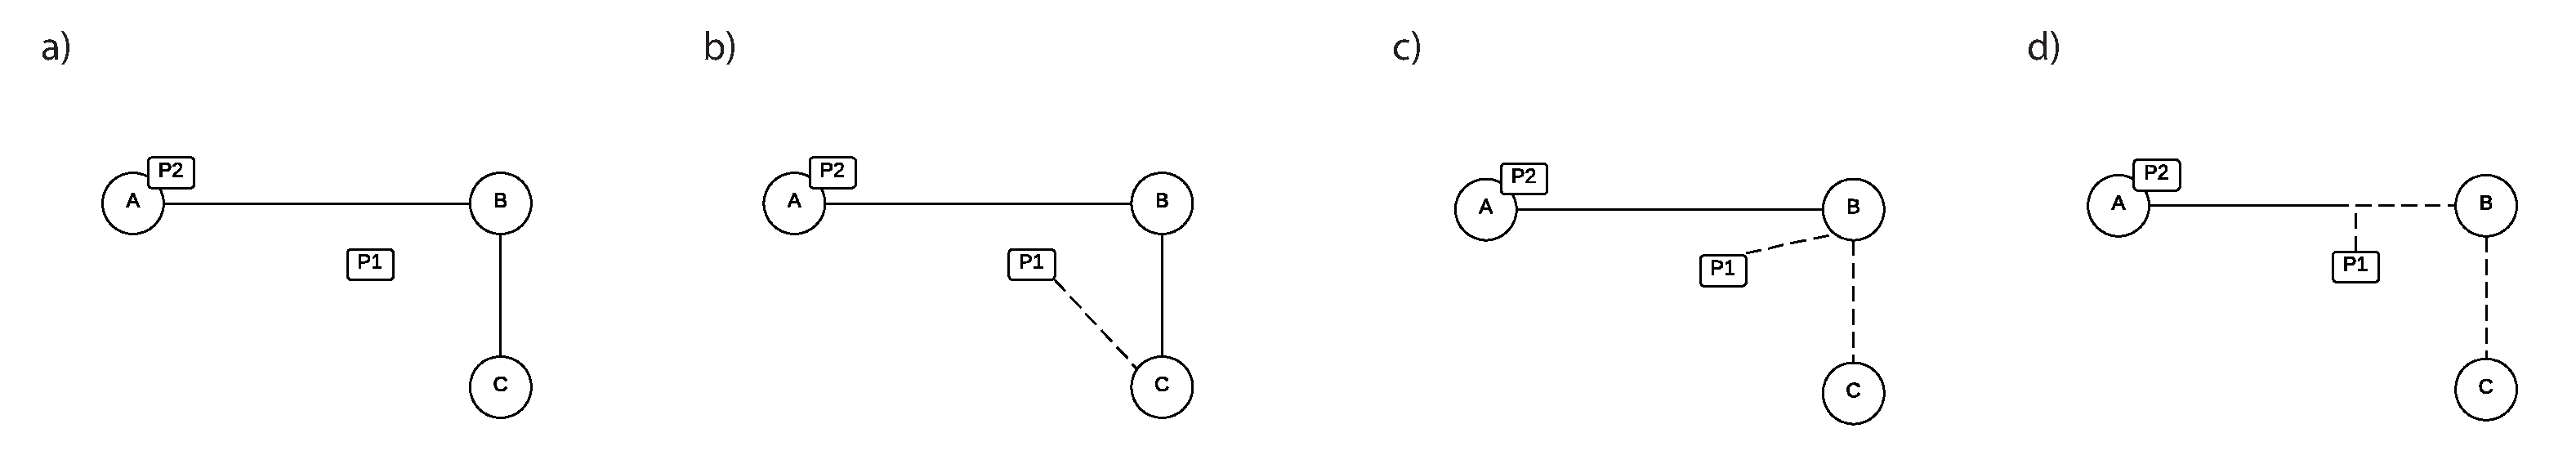
\includegraphics{res/pathfinding/PathFindingExample.pdf}
	\caption[Potential ship routes]{Potential routes a ship could take to reach its destination.}
	\label{fig:pathfindingexample}
\end{figure*}

First a typical ingame situation was taken to be analysed for the possible routes that a ship could take. Figure~\ref{fig:pathfindingexample} shows such a scenario. Figure~\ref{fig:pathfindingexample} (a) shows the location of two ships, $P_1$ and $P_2$, and three planets, $A$, $B$, and $C$, connected by spacelanes. If both ships want to reach planet $C$ then it is obvious which route $P_2$ will take, it can travel along spacelanes from $A$ to $B$ to $C$. However, there are three different possibilities for ship $P_1$:

\begin{enumerate}
	\item Go directly to planet $C$, shown in (b).
	\item Go to the closet planet, $B$, and then follow the spacelane to $C$, shown in (c).
	\item Travel to the nearest spacelane, between $A$ and $B$, and then follow the spacelanes to $C$, shown in (d).
\end{enumerate}

Travelling across open space is always going to be considerably slower than using spacelanes, so option one can be immediately be discarded as suboptimal. However, how fast are spacelanes? Is it best to greedily use spacelanes as much as possible or is it sometimes faster to travel a little longer through open space to reach a spacelane closer to the destination. Spacelanes have a multiplier effect on the speed of a ship so that a ship travelling along a spacelane speeds up $x$ times compared to its usual speed, where $x$ is a parameter defined by the sector model.

Suppose that $x$ is very large or infinite then travel along spacelanes with be almost instantaneous. Under these circumstances option three will be the optimal route since the least time is spent travelling off of spacelanes. However, for a lower value of $x$, option two will be optimal since the reduced distance to reach planet $B$ outweighs the benefits of the spacelane. Therefore, it is obvious that the heuristic cost function used by A* must take the multiplier effect of the spacelanes into account:

\begin{equation*}
	cost = \frac{distance}{speed \times multiplier}
\end{equation*}

Where the $distance$ between two nodes is simply the Euclidean distance. Using this cost function it becomes easier to find a good route by adding `virtual nodes' to the graph on nearby spacelanes and then using the A* algorithm to compare the costs of this extended graph. For example, in the scenario shown in Figure~\ref{fig:pathfindingexample} a virtual node is added to the spacelane between $A$ and $B$. This suggests a simple set of rules for adding new nodes:

\begin{enumerate}
	\item If the start point is in open space then add a node at the closest point on the closest spacelane
	\item If the destination is in open space then add a node at the closest point on the closest spacelane
\end{enumerate}

\begin{marginfigure}
	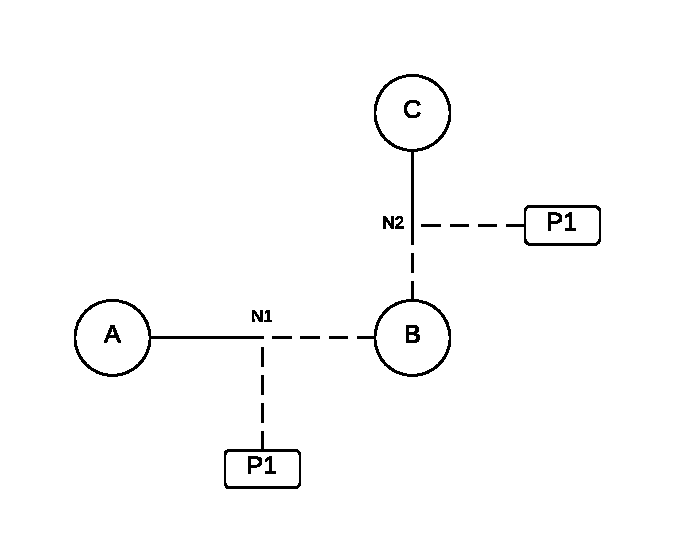
\includegraphics{res/pathfinding/PathFindingSector3.pdf}
	\caption[Adding nodes to the nearest spacelanes]{Adding nodes to the nearest spacelanes.}
	\label{fig:addingnodes}
\end{marginfigure}

For example, Figure~\ref{fig:addingnodes} shows how two nodes are added at $N_1$ and $N_2$ if a ship wants to go from $P_1$ to $P_2$. The graph is then completed to make all of the sensible routes connected. Using the same example from Figure~\ref{fig:addingnodes} it means that edges will be added between the $P_1$ and $N_1$, $P_2$ and $N_2$, $P_1$ to $B$, $B$ to $P_2$, and so on. The A* algorithm, using the simple cost function, can then be applied to this fully connected graph to find the best possible route to the destination.

\begin{marginfigure}
	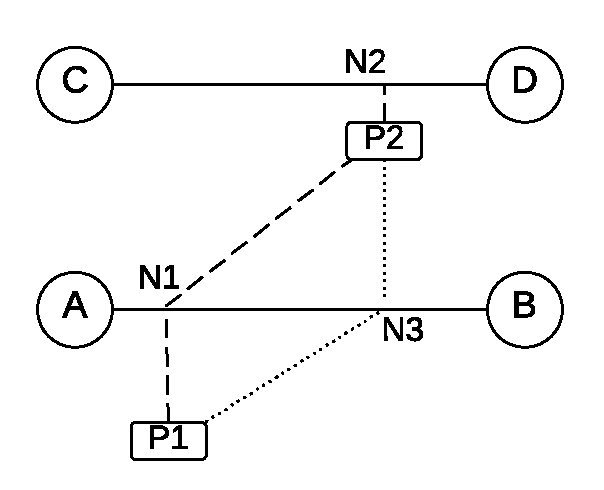
\includegraphics{res/pathfinding/NearestSpaceLaneUseless.pdf}
	\caption[The closest point on the closest spacelane is not always your friend]{The closest point on the closest spacelane is not always your friend.}
	\label{fig:uselessspacelane}
\end{marginfigure}

However, these two rules are too simplistic and will not provide the best route in all cases. Figure~\ref{fig:uselessspacelane} shows an example in which a ship wants to travel from $P_1$ to $P_2$. The current ruleset will add nodes $N_1$ and $N_2$ since they are the closest points on the nearest spacelanes. However, it is actually quicker to travel via $N_3$ than it would be to go straight from $N_1$ to $P_2$. There are just too many possibilities for quicker routes as the edge cases keep on building up. Therefore, it was decided to use a brute force solution that involves adding nodes at regular intervals along the nearest spacelanes. The best added node may not match the optimal solution exactly, but it will be better than the majority of other options. Using brute force is also not a highly desirable technique, but it works fast enough for this use case for now as further designing would have been required to reach a better solution.

Now that a discrete graph has been generated to represent the sector it can be fed to the A* algorithm which will find an optimal solution for the graph it has been presented.

\clearpage\section{Assets}


% ships made to look very big
% many prototypes
% merging assets with code, dynamic color
% colour selection algorithm http://gamedev.stackexchange.com/questions/46463/is-there-an-optimum-set-of-colors-for-10-players


% master copy of assets in dropbox under 4y project/laith/design
% 
\section{Configuration}

% defining weapons, systems, ship classes, and fleets externally.
% information defined in yaml
% 

This section describes the method used to defines the various weapons, systems, ship classes, and fleets.
For simplicity, The weapons, systems, ship classes, and fleets will be referred to as Addons.
The reason for this name is that to add a new weapon, system, etc should be very easy from a development point of view.

Their were two options for this: defining the Addons within the code, or defining them in external resources and loading them in at runtime.
The second option is a cleaner and simpler design and allows new Addons to be defined without changing the code.

There are many data serialisation formats that are designed for this in mind, such as: XML, JSON, and YAML.
XML is highly verbose for both reading and writing, JSON requires braces for scope and quotes for any strings whereas YAML doesn't need either since it uses the white space for scoping and strings don't need quotes.
YAML is also designed to be human readable and writable, which would make manually creating and editing these Addons very easy.

It was important that new Addons should be discovered by the game when it loads, i.e. it would search for them in a given directory.
It would make the logic a little more complex but would make the interactions with the Addons very simple.
If you wanted to add an Addon simply add the a new yaml file to the correct directory, if you wanted to edit an Addon simply find the yaml file and change what values you wanted.
Unfortunately deleting Addons is not so simply, because some Addons will have dependencies on other Addons, for example a fleet may use a certain ship class, and if that ship class was deleted, that fleet would no longer be usable.
Making the deletion of Addons simple was considered, but decided against it because it would require disabling all Addons that had a dependency on a deleted Addon. This wasn't a clean design hence it is typically assumed that either no Addons are deleted or that the user knows what they are doing.
An example of a ship class defined in yaml is provided in Figure \ref{fig:configuration:corvetteYaml}


\begin{marginfigure}
	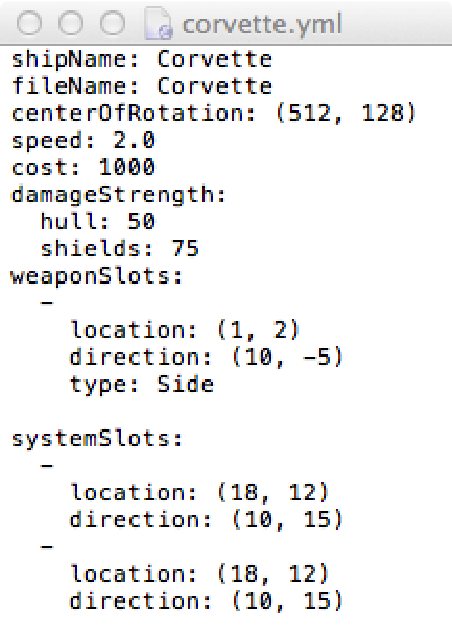
\includegraphics{res/configuration/corvetteYaml.pdf}
	\caption{
	example of ship class defined in yaml
	}
	\label{fig:configuration:corvetteYaml}
\end{marginfigure}




    
\begin{comment}

story boards:
  - client/server updates loop
  - graphics:
    - navigation
    - Paralex
  - GUI interfaces: 
    - Main Menu
    - credits
    - Game Play 
    - fleet design 
    - Results Screen
  - resources
  - planet capture
  - ship weapons arcs
  - model (sector, ship, etc)
  - AI concepts (PLAN/GOAL/ORDER)
  - path finding
    - A*
    - Bezier path
    - Flow fields
  - assets and configuration
    - assets
    - asset meta data
    - fleets
  - future work sections...
  - conclude (something)
  

\end{comment}


\begin{comment}

overall layout
--------------
game decisions
where we got to in spec
current state of game
lots of pictures

very little technical detail

lot of work on infrastructure at start



layout:
- laying the foundations:
    - got infrastructure sorted out:
        - network
        - overall glue
- alpha stage (Christmas):
    - demo stage
- leading beta stage:
    - messages/updates
    - better graphics
    - AI
- current state
- play testing and feedback
    - LIE we did lots
- future work(ryan's mum)


\end{comment}


